% This is a LaTeX thesis template for Adam Mickiewicz University.
% to be used with Rmarkdown
% This template was produced by Jakub Nowosad
% Version: 16 February 2020

% Inspired by:
% This is a LaTeX thesis template for Monash University.
% to be used with Rmarkdown
% This template was produced by Rob Hyndman
% Version: 6 September 2016

\documentclass{amuthesis}
\usepackage[polish]{babel}
\usepackage{polski}
\usepackage{caption}
\captionsetup[figure]{name=Rycina}
\renewcommand{\figurename}{Rycina} % Redefine default figure caption %
\renewcommand{\tablename}{Tabela} % Redefine default table caption %
%%%%%%%%%%%%%%%%%%%%%%%%%%%%%%%%%%%%%%%%%%%%%%%%%%%%%%%%%%%%%%%
% Add any LaTeX packages and other preamble here if required
%%%%%%%%%%%%%%%%%%%%%%%%%%%%%%%%%%%%%%%%%%%%%%%%%%%%%%%%%%%%%%%
\usepackage{booktabs,tabularx} % Allows kableExtra to work %
\usepackage{indentfirst} % Adds indent in the first paragraph %

\author{Kacper Misiun}
\title{Analiza wykorzystania roweru miejskiego w Kołobrzegu w kontekście dokumentów strategicznych miasta}
\def\titleeng{Analysis of the rentals of the Kolobrzeg City Bicycle in context of strategic reports in 2021}
\def\degreetitle{Praca inżynierska}
\def\major{Zintegrowane Planowanie Rozwoju}
\def\albumid{414342}
\def\thesisyear{2022}
% Add subject and keywords below
\hypersetup{
     %pdfsubject={The Subject},
     %pdfkeywords={Some Keywords},
     pdfauthor={Kacper Misiun},
     pdftitle={Analiza wykorzystania roweru miejskiego w Kołobrzegu w kontekście dokumentów strategicznych miasta},
     pdfproducer={Bookdown with LaTeX}
}

\bibliography{thesis,packages}

\begin{document}

\pagenumbering{arabic}

\titlepage

\newpage
\setlength\parindent{24pt}

\hfill Poznań, dnia \ldots\ldots\ldots.

\begin{center}
\large{\textbf{OŚWIADCZENIE}}
\end{center}

\indent Ja, niżej podpisany/a student/ka Wydziału Geografii Społeczno-Ekonomicznej i Gospodarki Przestrzennej Uniwersytetu im. Adama Mickiewicza w Poznaniu oświadczam, że przedkładaną pracę dyplomową napisałem/napisałam samodzielnie. Oznacza to, że przy pisaniu pracy, poza niezbędnymi konsultacjami, nie korzystałem/am z pomocy innych osób, a w szczególności nie zlecałem/am opracowania rozprawy lub jej części innym osobom, ani nie odpisywałem/am tej rozprawy lub jej części od innych osób. \newline
\indent Oświadczam również, że egzemplarz pracy dyplomowej w wersji drukowanej jest całkowicie zgodny z egzemplarzem pracy dyplomowej w wersji elektronicznej. \newline
\indent Jednocześnie przyjmuję do wiadomości, że przypisanie sobie, w pracy dyplomowej, autorstwa istotnego fragmentu lub innych elementów cudzego utworu lub ustalenia naukowego stanowi podstawę stwierdzenia nieważności postępowania administracyjnego w sprawie nadania tytułu zawodowego.

{[}\hspace{0.6cm}{]}* - wyrażam zgodę na udostępnianie mojej pracy w czytelni Archiwum UAM

{[}\hspace{0.6cm}{]}* - wyrażam zgodę na udostępnianie mojej pracy w zakresie koniecznym do ochrony mojego prawa do autorstwa lub praw osób trzecich

\vspace{5mm}

\begin{footnotesize}
*Należy wpisać TAK w przypadku wyrażenia zgody na udostępnianie pracy w czytelni Archiwum UAM, NIE w przypadku braku zgody. Niewypełnienie pola oznacza brak zgody na udostępnianie pracy.
\end{footnotesize}

\vspace{20mm}

\hfill\ldots\ldots\ldots\ldots\ldots\ldots\ldots\ldots\ldots\ldots\ldots\ldots\ldots\ldots\ldots. \newline
\null\hfill

\begin{scriptsize}(czytelny podpis studenta)\end{scriptsize}

\newpage

\hypertarget{streszczenie}{%
\section*{Streszczenie}\label{streszczenie}}
\addcontentsline{toc}{section}{Streszczenie}

Głównym celem pracy jest analiza Kołobrzeskiego Roweru Miejskiego w kontekście generowanego przez rower miejski natężenia ruchu rowerowego w poszczególnych stacjach oraz analiza dokumentów strategicznych w Kołobrzegu.
Analizę natężenia rowerowego wykonano między innymi za pomocą języka R, a dane pobrano za pośrednictwem Nextbike API.
Analiza dokumentów strategicznych obejmowała analizę studium uwarunkowań i kierunków zagospodarowania przestrzennego, strategie rozwoju SmartCity oraz analizę SWOT dotyczącą polityki przestrzennej i infrastruktury rowerowej.
Ponadto przeprowadzono badanie ankietowe na próbie ponad 100 osób dotyczące roweru miejskiego w Kołobrzegu i kołobrzeskiej infrastruktury rowerowej oraz przedstawiono charakterystykę miasta Kołobrzeg,

Wynikiem analiz jest projekt koncepcji zagospodarowania, która zakłada powstanie nowych stacji Kołobrzeskiego Roweru Miejskiego, które przedstawiono na mapach wykonanych za pomocą oprogramowania QGis oraz za pośrednictwem platformy System Informacji Przestrzennej Miasta Kołobrzeg.

Słowa kluczowe: System roweru publicznego, infrastruktura rowerowa, badanie ankietowe, SmartCity, język R

\hypertarget{abstract}{%
\section*{Abstract}\label{abstract}}
\addcontentsline{toc}{section}{Abstract}

The main aim of this paper is to analyse Kolobrzeg's Urban Bicycle in the context of bicycle traffic generated by the bicycle at individual stations and to analyse strategic documents in Kolobrzeg.
The analysis of the bicycle traffic volume was performed using the R language, among others, and the data was downloaded via Nextbike API.
The analysis of strategic documents included an analysis of the spatial development conditions and directions, SmartCity development strategies, and a SWOT analysis of spatial policy and cycling infrastructure.
In addition, a survey was carried out on a sample of more than 100 people on urban cycling in Kołobrzeg and the Kołobrzeg cycling infrastructure, and the characteristics of the city of Kołobrzeg were presented,

The result of the analyses is a draft development concept, which assumes the creation of new Kolobrzeg City Bicycle stations, which are presented on maps created using the QGis software and via the Spatial Information System platform of the City of Kolobrzeg.

Keywords: Bike-sharing system, bicycle infrastructure, questionnaire survey, SmartCity, R language

\newpage

\setstretch{1.2}\sf\tighttoc\doublespacing

\hypertarget{wprowadzenie}{%
\chapter{Wprowadzenie}\label{wprowadzenie}}

\hypertarget{cel}{%
\section{Cel i zakres pracy}\label{cel}}

Celem pracy jest przedstawienie analizy natężenia ruchu rowerowego w poszczególnych stacjach Kołobrzeskiego Roweru Miejskiego, analiza dokumentów strategicznych wraz z poglądowym opisem charakterystyki miasta Kołobrzeg oraz prezentacja wniosków z ankiety przeprowadzonej wśród mieszkańców i osób odwiedzających miasto Kołobrzeg. Na podstawie analiz opracowano projekt koncepcji nowych stacji Kołobrzeskiego Roweru Miejskiego oraz zasugerowano stacje w których należy zwiększyć przepustowość ruchu rowerowego.

Zakres przestrzenny podjętych analiz obejmuje gminę miejską Kołobrzeg.
Przedział czasowy pracy badawczej obejmuje sezon rowerowy 2021 i obejmuje czas działania Kołobrzeskiego Roweru miejskiego, który funkcjonuje od marca do listopada.

W celu opracowania analizy natężenia ruchu w poszczególnych stacjach, najczęściej wybieranych kierunków oraz przedstawienia ogólnego natężenie ruchu rowerowego generowanego przez Kołobrzeski Rower Miejski, opierając się na danych udostępnionych przez operatora Kołobrzeskiego Roweru Miejskiego stworzono wykresy przedstawiające rozkład ilości wypożyczeń w zależności od miesiąca lub pory roku dla poszczególnych dni tygodnia, wypożyczenia przychodzące i wychodzące w zależności od pory dnia dla poszczególnych stacji oraz najczęściej występujące kierunki przemieszczeń w zależności od pory dnia w poszczególne pory roku.

\hypertarget{zrodl}{%
\section{Materiały, metody i narzędzia badawcze}\label{zrodl}}

Dane poddane analizie pochodzą od operatora Kołobrzeskie Roweru Miejskiego, firmy Nextbike Polska, który jest częścią niemieckiego koncernu Nextbike.
Są one dostępne są na stronie operatora i zostały pozyskane za pomocą skryptu w języku python, który pobierał dane o lokalizacji rowerów w interwale 2 minutowym.
Dane opracowane w niniejszej pracy zostały pozyskane w powyższy sposób przez doktora Michała Dzięcielskiego.
Pozyskane w ten sposób dane poddano transformacji oraz eksploracji za pomocą języka R.
W tym celu wykorzystano następujące biblioteki:

\begin{itemize}
\item
  \emph{readr} \autocite{R-readr}
\item
  \emph{plm} \autocite{R-plm}
\item
  \emph{ggplot2} \autocite{R-ggplot2}
\item
  \emph{data.table} \autocite{R-data.table}
\item
  \emph{ggTimeSeries} \autocite{R-ggTimeSeries}
\item
  \emph{cowplot} \autocite{R-cowplot}
\item
  \emph{plyr} \autocite{R-plyr}
\item
  \emph{dplyr} \autocite{R-dplyr}
\item
  \emph{tidyr} \autocite{R-tidyr}
\item
  \emph{geosphere} \autocite{R-geosphere}
\end{itemize}

Ankiety opracowano kierując się zasadami badania sondażowego i konstrukcji kwestionariusza zgodnie z zasadami nauk społecznych (za \textcite{nachmias}) za pomocą Microsoft Forms i udostępniono za pośrednictwem internetu na portalu społecznościowym Facebook.

Analizę przestrzenną oraz opracowanie map wykonano za pomocą oprogramowania geoinformacyjnego QGIS, społecznościowego serwisu GIS OpenStreetMap oraz korzystając z serwisów mapowych za pośrednictwem platformy System Informacji Przestrzennej Miasta Kołobrzeg.

\hypertarget{ogolny}{%
\chapter{Ogólna charakterystyka miasta}\label{ogolny}}

\hypertarget{historia}{%
\section{Historia miasta}\label{historia}}

Osadnictwo na terenie obecnego Kołobrzegu sięga VII wieku, kiedy to powstała osada na Wyspie Solnej, gdzie pozyskiwano sól ze źródeł solankowych.
Była ona źródłem bogactwa okolicznej ludności, dzięki czemu w IX wieku przystąpiono do budowy grodziska na terenie obecnego Budzistowa (wieś na południowych obrzeżach miasta Kołobrzeg).
Miasto jest wspominane w kronikach Thietmara jako Solny Kołobrzeg (Salsae Colbergiensis), podkreśla to \emph{solny rodowód} miasta.

Badania archeologiczne wskazują, że do X wieku grodzisko przekształciło się w ufortyfikowany gród o charakterze wczesnomiejskim \autocite{historia_kołobrzeg}, który był ważnym ośrodkiem polityczno-gospodarczym na wschód od ujścia Odry a na zachód od ujścia Wisły.
Świadczy o tym ustalenie na zjeździe gnieźnieńskim diecezji kołobrzeskiej w 1000 roku, która podporządkowana metropolii gnieźnieńskiej obejmowała całe Pomorze i jak wskazuje nazwa siedziba diecezji znajdowała się w Kołobrzegu.
Działalność misyjna połączona była z próbą utrwalenia zwierzchnictwa państwa Piastów nad Pomorzem Zachodnim.
Działania te nie przyniosły rezultatu i państwo Polskie utraciło zwierzchność nad Pomorzem Zachodnim w 1007 roku, tym samym przerywając działalność misjonarską (a co za tym idzie cywilizacyjną, mającą wpływ na kształt wczesnośredniowiecznego Kołobrzegu) aż do ponownego podporządkowania tych terenów przez Bolesława Krzywoustego w pierwszej połowie XII wieku.
W okresie rozbicia dzielnicowego Kołobrzeg znalazł się pod panowaniem duńskim, żeby następnie odzyskać niezależność pod władzą książąt pomorskich.

W 1255 roku książe pomorski Warcisław III lokował nowe miasto bliżej wybrzeża na prawie lubeckim.
Dawny gród opuszczono a w pamięci przyszłych pokoleń teren ten został zapamiętany jako Stare Miasto (\emph{Altstat}) \autocite{historia_kołobrzeg_wiki}.
Część osadników zagospodarowujących nową przestrzeń miejską pochodziło ze Starego Kołobrzegu, jednak sporą część nowych mieszkańców stanowili imigranci z miast hanzeatyckich - głównie z Gryfii (\emph{Greifswald}), Lubeki i Brunszwiku.
Napływ ludności niemieckojęzycznej spowodował że w okresie następnych 100 lat nastąpiła asymilacja rodzimej ludności słowiańskiej.
Nastąpiło przyjęcie nowych wzorców kulturowych, upowszechnienie się zachodnich rozwiązań technologicznych, gospodarczych i prawnych.
Nowe miasto założono na prawie lubeckim dlatego też początkowo w kołobrzeskim sądzie rozpatrywano jedynie sprawy w pierwszej instancji (apelacje składano do Gryfii, kasacje do Lubeki) jednak gdy liczba spraw w Kołobrzegu zaczęła wzrastać dokonano odpisu Kodeksu Prawa Lubeckiego i przywieziono go (odpis kodeksu) w uroczystych okolicznościach do miasta.
Co ciekawe Kołobrzeski odpis Kodeksu Prawa Lubeckiego liczy 192 artykuły z oryginalnych 237.
Kodeks ten obowiązywał formalnie do 1 czerwca 1794 roku.

\begin{figure}[t]

{\centering \includegraphics[width=400px]{figures/widok_miasto} 

}

\caption{Hipotetyczny widok Kołobrzegu na początku XV w. autorstwa J. Tężyckiego i M. Rębkowskiego. (Źródło: Robert Dziemba, Historia Kołobrzegu dla średniozaawansowanych, 2018)}\label{fig:ryc7}
\end{figure}

W okresie średniowiecza, miasto regularnie się rozbudowywało.
Jeszcze pod koniec XIII wieku rozpoczęto realizację monumentalnej inwestycji, jaką była budowa kolegiaty.
Pierwszy ratusz powstał przy ul. Podgórnej (obecnie ulica Wąska).
Wiek później drewnianą zabudowę zaczęto zastępować zabudową murowaną.
Osuszono prawy brzeg Parsęty (ulica Rzeczna), na który przeszła ekspansja tkanki miejskiej.
Zbudowano mur obronny długości ponad 1500 metrów wraz z dwiema basztami.
Wzmocniło to poczucie bezpieczeństwa mieszkańców, choć dzięki położeniu geograficznemu Kołobrzeg posiada naturalnie dobre warunki do obrony, od południa miasto chroniła rzeka, a od wschodu rozległe bagniska i tereny podmokłe.

W średniowieczu miasto bogaciło się na handlu solą, którą importowano zwłaszcza do północnej Wielkopolski.
W XII i XIII wieku zmieniła się struktura własnościowa salin kołobrzeskich.
Początkowo duży udział w warzelniach miały klasztory i istytucje kościelne, jednak do 1300 roku, kiedy to powstało pierwsze na tych ziemiach bractwo solne głównymi właścicielami warzelni stali się mieszkańcy \autocite{heider}.
W XV wieku, Kołobrzeg stał się potęgą gospodarczą nad Bałtykiem, uzależniając od siebie inne mniejsze miasta.

Okres prosperity trwał do wojny trzydziestoletniej (\emph{1618-1648}).
Mimo prób zachowania neutralności w tym konflikcie Księstwo Pomorskie stało się areną działań wojennych w 1627 roku, kiedy to uległo i zgodziło się na zakwaterowanie wojsk cesarskich.
Rozpoczęło to okupacje miasta, która spustoszyła miasto.
Doprowadziło to do samowoli żołnierzy, którzy dopuszczali się gwałtów, rabunków i podpaleń.
W 1630 roku od czerwca do września w mieście wybuchła zaraza, która zabiła 3,5 tysiąca ludzi.
Na domiar złego we wrześniu tego samego roku wybuchł wielki pożar, który pochłonął południowo-zachodnią część miasta.
O rozmiarze trudów z jakimi zmagali się mieszkańcy świadczy radość z jaką powitali w 1631 roku okupacje szwedzką miasta, po kapitulacji garnizonu wojsk cesarskich.
Szwedzi przystąpili do fortyfikacji Kołobrzegu, tworząc na zewnątrz średniowiecznych
murów wielobok bastionowy.
Książe pomorski Bogusław XIV zmarł bezpotomnie i w wyniku pokoju westfalskiego, kończącego wojne trzydziestoletnią podzielono Księstwo Pomorskie na Pomorze Przednie, które przypadło szwedom oraz na Pomorze Przednie, które otrzymał elektor brandenburski.
Kołobrzeg będący enklawą szwedzką w wyniku rokowań przeszedł pod władze Brandenburgii dopiero 5 lat po zakończeniu wojny.
Kołobrzeg dekretem zamieniono w twierdze i przez następne lata rozbudowano fortyfikacje oraz port morski, będący portem macierzystym floty brandenburskiej.

\begin{figure}[t]

{\centering 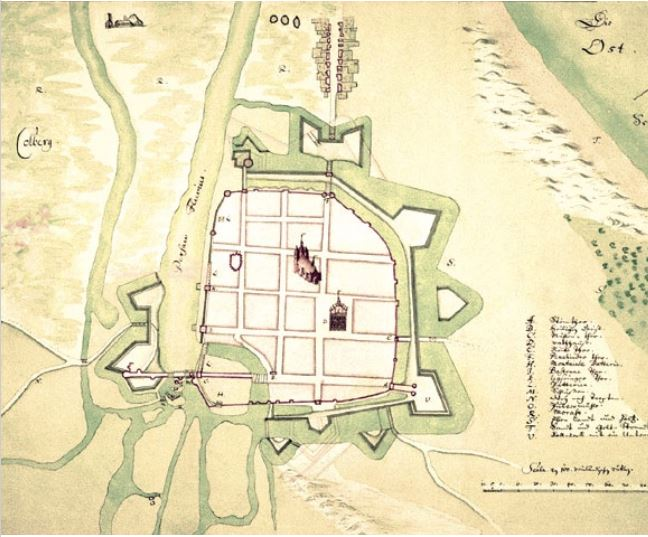
\includegraphics[width=400px]{figures/plan_twierdzy_kolobrzeg_1687} 

}

\caption{Plan twierdzy kolobrzeg 1687 (Źródło:https://twierdzakolobrzeg.pl)}\label{fig:ryc1}
\end{figure}

Od tej pory Kołobrzeg jako twierdza był świadkiem najważniejszych konfliktów zbrojnych w Europie.
Podczas wojny siedmioletniej (1756--1763), Kołobrzeg był trzykrotnie oblegany przez Rosjan (trwała także blokada morska miasta).
Zdobyli oni miasto pod koniec 1761 roku i przez pół roku okupowali miasto, mimo zniszczeń wojennych dobrze zapisując się w pamięci mieszkańców \autocite{historia_kołobrzeg}.
Kołobrzeg w 1762 roku \emph{wrócił} pod władanie Pruskie i w następnych latach poczyniono znaczne inwestycje w rozbudowanie nowoczesnych fortyfikacji.

\begin{figure}[t]

{\centering \includegraphics[width=400px]{figures/twierdza_koł} 

}

\caption{Plan twierdzy Kołobrzeg po rozbudowie w 1770 roku (Źródło:https://twierdzakolobrzeg.pl)}\label{fig:ryc2}
\end{figure}

Podczas wojen napoleońskich twierdza w Kołobrzegu stała się symbolem oporu, kiedy to po klęskach armii pruskiej pod Jeną i Auerstädt oraz po upadku Berlina załoga twierdzy Kołobrzeg odmówiła kapitulacji i przez 4 miesiące skutecznie broniła się.
SKutkowało to dużymi zniszczeniami w mieście, ale wydarzenia te stały się później ważnym niemieckim symbolem narodowym.

\begin{figure}[t]

{\centering 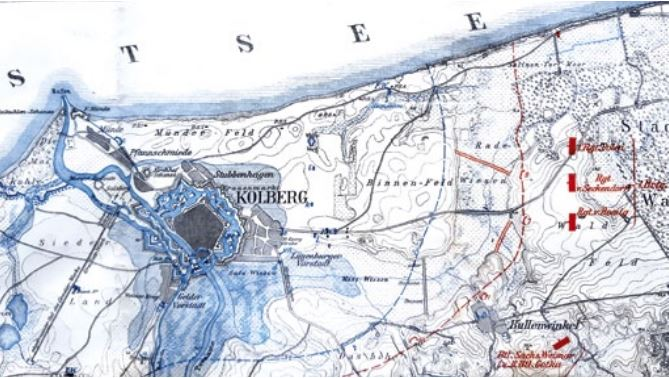
\includegraphics[width=400px]{figures/Kolobrzeg_napoleon} 

}

\caption{Plan oblężenia Twierdzy Kołobrzeg w 1807 roku (Źródło:https://twierdzakolobrzeg.pl)}\label{fig:ryc3}
\end{figure}

Po 1807 roku nastąpiła ponowna odbudowa miasta, przy czym priorytetem była odbudowa fortyfikacji.
Zmodernizowano sposób produkcji w Kołobrzeskich warzelniach soli, które od 1801 roku należały do pruskiego rządu.
Mimo starań rządu produkcja soli z solanki w Kołobrzegu okazała się nierentowna i w 1858 roku zlikwidowano produkcje soli, kończąc wielowiekową tradycje warzelnictwa.
Jednak nie był to koniec wpływu soli na rozwój miasta.
Już w 1803 roku powstał Zakład Kąpieli Morskich i w kolejnych latach powstały domy zdrojowe dla kuracjuszy.
Dlatego też, kilka lat po zlikwidowaniu warzelni źródła solankowe przekazano do dyspozycji uzdrowiska \autocite{heider}.

W latach 1832--1836 przeprowadzono ostatnią wielką modernizację fortyfikacji Twierdzy Kołobrzeg.
Zbudowano także istniejący po dziś dzień neogotycki ratusz, zaprojektowany przez wybitnego niemieckiego architekta Karla Friedricha Schinkela.

W 1873 podjęto decyzje o likwidacji twierdzy Kołobrzeg, 15 lat później podjęto decyzje o likwidacji morskiej Twierdzy Kołobrzeg.
Oznaczało to przejęcie gruntów, które należały do wojska przez władze miejskie.
Przez następne 30 lat trwał proces przekształcania Kołobrzegu w ``standardowe'' miasto. Zniwelowano wały forteczne, zasypano fosy i na ich miejsce wytyczono nowe ulice.
Zabudowania forteczne, których nie rozebrano otrzymały funcke kulturalną, gastronomiczną, mieszkalną lub pamiątkową \autocite{historia_kołobrzeg}.
Decyzja ta wpłynęła pozytywnie na rozwój funkcji uzdrowiskowej miasta, wraz z wytaczaniem nowych ulic powstawały zakłady zdrojowe, kurorty i pensjonaty.

Podczas I wojny światowej, działania wojenne ominęły Kołobrzeg.
Na czas wojny w mieście zorganizowano zaplecze medyczne.
Mimo, że miasto nie ucierpiało w wyniku walk to sytuacja Kołobrzegu po wojnie była trudna.
Podupadła gospodarka, ponieważ zamarła branża turystyczna.
W przegranych Niemczech szerzyło się bezrobocie, bieda oraz hiperinflacja, która wpłynęła na sytuacje mieszkańców ówczesnego Kołobrzegu.

Podczas II wojny światowej Kołobrzeg ponownie w swojej historii został mianowany twierdzą.
Miasto zostało umocnione i zbudowano system barykad.
W dniach 4--18 marca 1945 roku stoczono krwawą bitwę o Kołobrzeg.
Bitwa miała charakter walk miejskich i w jej wyniku zniszczono Kołobrzeg w 80-95\% w zależności od źródeł.

\begin{figure}[t]

{\centering 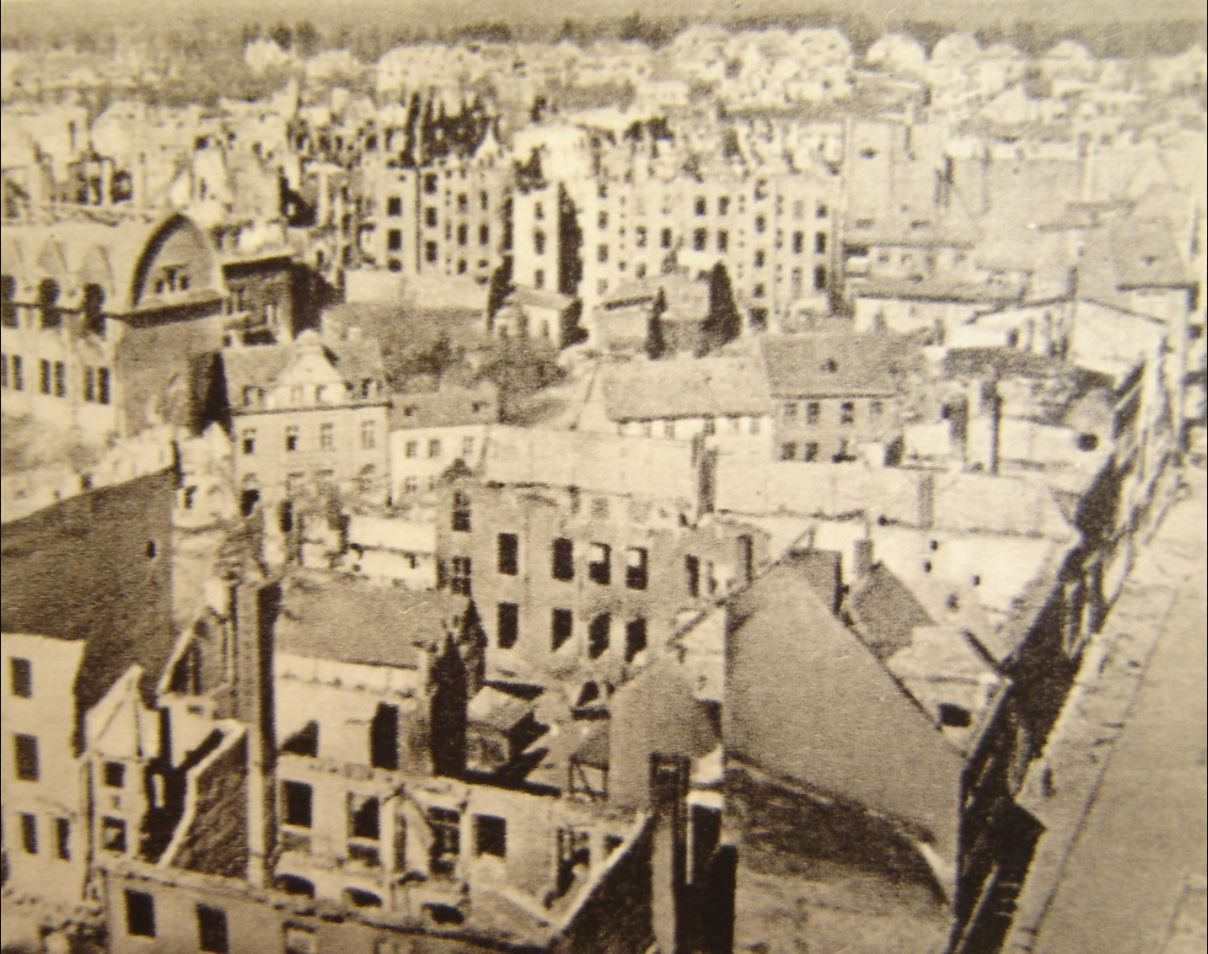
\includegraphics[width=400px]{figures/kolobrzeg_wojna} 

}

\caption{Widok na Kołobrzeg w 1945 roku (Źródło:https://twierdzakolobrzeg.pl)}\label{fig:ryc4}
\end{figure}

W okresie od zdobycia miasta w marcu do 31 maja -kiedy to miasto przekazano polskim władzom - dokonywano zorganizowanego rabunku mienia i wywozu majątku pozostawionego przez mieszkańców.
Jeszcze miesiąc po zakończeniu walk miasto wciąż spowijała łuna pożarów.
Grabież tak wspomina Ludwik Herczak-Osmoliński, który był był w Kołobrzegu 20 kwietnia 1945 roku (\textcite{kołobrzeg_cytat}):

\begin{quote}
``W parku stała nieobliczalna ilość sprzętu wojskowego, armat, czołgów, samochodów pancernych, amunicji. Wśród tego żelastwa walały się trupy żołnierskie i zabite konie. Przeskoczyliśmy wydmy i zobaczyliśmy pas wzburzonego morza. W pobliżu brzegu widać było zatopione okręty i stateczki niemieckie. Po kilku dniach rozejrzeliśmy się po mieście. Na ulicy Dworcowej, w gruzowiskach domów leżały dziesiątki trupów polskich żołnierzy. Nie mieli na sobie płaszczy, tylko drelichowe mundury i czapki polowe z orzełkami wojska Berlinga. Na ich nogach zobaczyłem parciane obuwie. Druga, duża grupa polskich żołnierzy leżała w piwnicach domu przy skrzyżowaniu ulicy Armii Krajowej i Łopuskiego. Naliczyłem ich przeszło osiemdziesiąt. Trupy ludności cywilnej i żołnierzy niemieckich walały się wszędzie, na ulicach i wokół domów, nikt ich nie uprzątnął.
Rosjanie buszowali w mieście. Na rampę kolejową, której dzisiaj już nie ma, a stała ona w miejscu dzisiejszych pawilonów handlowych przy ul. Kolejowej (kładka dla pieszych), dojeżdżały samochody ciężarowe i dowożono do towarowych wagonów dosłownie wszystko. Tę wywózkę łupów wojennych pilnowali żołnierze Armii Czerwonej. Wzdłuż ulicy Unii Lubelskiej stały w rzędach po jednej i drugiej stronie jezdni kombajny zbożowe, maszyny rolnicze, fortepiany, meble, maszyny do szycia i sprzęt gospodarczy. Było tego tysiące. Wywózka trwała bez przerwy''"
\end{quote}

\hypertarget{polozenie}{%
\section{Położenie (administracyjne, geograficzne)}\label{polozenie}}

Miasto Kołobrzeg jest gminą miejską położoną w północno-zachodniej części Polski, na Pomorzu Zachodnim, w północnej części województwa zachodniopomorskiego, w powiecie
kołobrzeskim.
Miasto Kołobrzeg stanowi gminę miejską Kołobrzeg i sąsiaduje z gmina wiejska o tej samej nazwie (Kołobrzeg) oraz od wschodu z gminą wiejską Ustronie Morskie.
Gmina miejska Kołobrzeg podzielona jest na 9 osiedli (patrz Rycina \ref{fig:ryc8}).

\begin{figure}[t]

{\centering 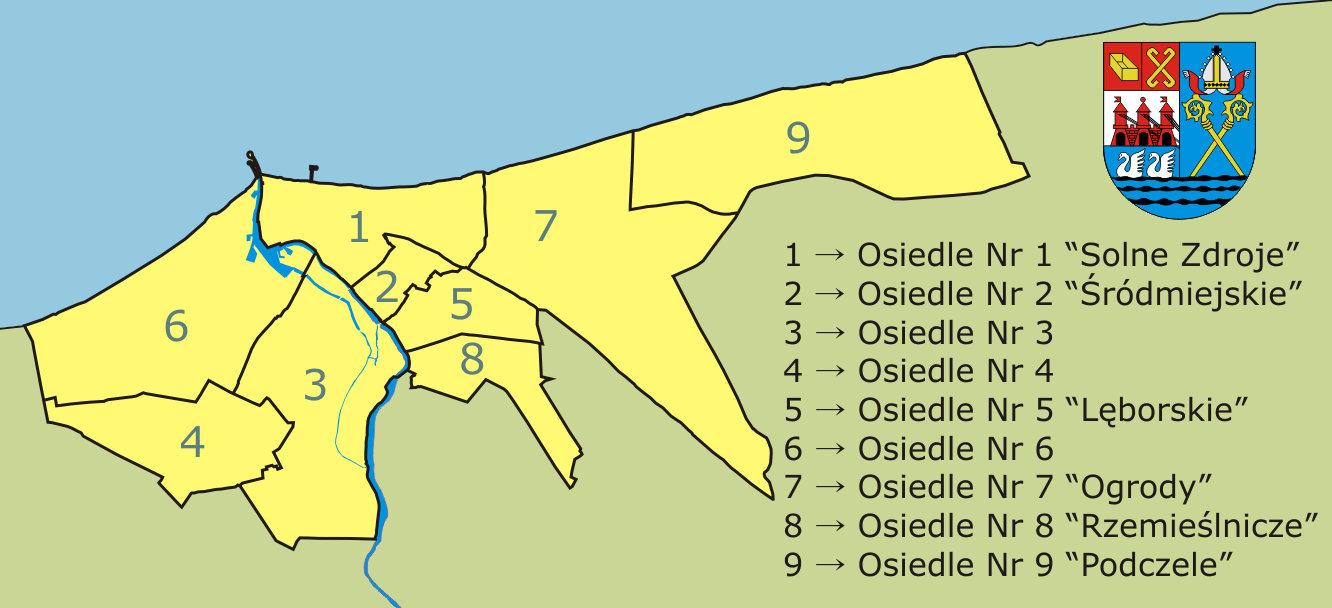
\includegraphics[width=1.05\linewidth]{figures/Kolobrzeg_administrative_division_2005} 

}

\caption{Podział administracyjny Kołobrzegu (Źródło: wikipedia.org)}\label{fig:ryc8}
\end{figure}

Jest miastem nabrzeżnym Morza Bałtyckiego, gdzie swe ujście ma rzeka Parsęta, która stanowi naturalną granicę rozdzielającą strefę brzegową Wybrzeża Trzebiatowskiego i Wybrzeża Słowińskiego.
Rzeźba terenu wznosi się w górę w kierunku południowym, a krajobraz jest urozmaicony dzięki dolinie rzecznej Parsęty.
Na terenie gminy miejskiej naturalnie dominują gleby torfowe i bielicowe, natomiast w strefach zurbanizowanym występują zwarte gleby o charakterze antropogenicznym (usypiska, sztucznie zasilane plaże i urbisole).

\hypertarget{przyr}{%
\section{Środowisko przyrodnicze}\label{przyr}}

Miasto Kołobrzeg w dokumentach planistycznych i strategicznych uwzględnia aspekt środowiskowy.
Efektem działań władz lokalnych jest rozwój terenów zielonych, na przestrzeni dekady (2009- 2019) ich udział w ogólnej powierzchni zwiększył się niemal dwukrotnie (5,1\% do 9\%).
Jednocześnie gospodarczy i turystyczny rozwój Kołobrzegu wywiera istotną presję na
system przyrodniczy miasta i jakość środowiska.
Kurczą się zasoby przestrzeni miasta, a lokalny system przyrodniczy poddawany jest coraz większej presji ze strony przybywających turystów (\textcite{smartcity}).

Ekopark Wschodni znajduje się we wschodniej części miasta, na terenach leśnych oddzielających Kołobrzeg od osiedla Podczele.
Teren ten był dawniej administrowany przez wojsko, natomiast od 1996 został powołany ekopark i jest częścią Trzebiatowsko-Kołobrzeskiego Pasa Nadmorskiego.
Obejmuje 381 hektarów na których znajdują się unikalne solne torfowiska zamieszkane przez wyjątkowe gatunki zwierząt i roślin.
Teren parku jest ważną ostoją ptaków, gniazduje tu i żeruje ok 100 gatunków ptaków, takich jak bąk, rybołów, czapla biała, żuraw, rybitwa rzeczna, gęś gęgawa czy łabędź niemy (\textcite{ekopark}).

\begin{figure}[t]

{\centering 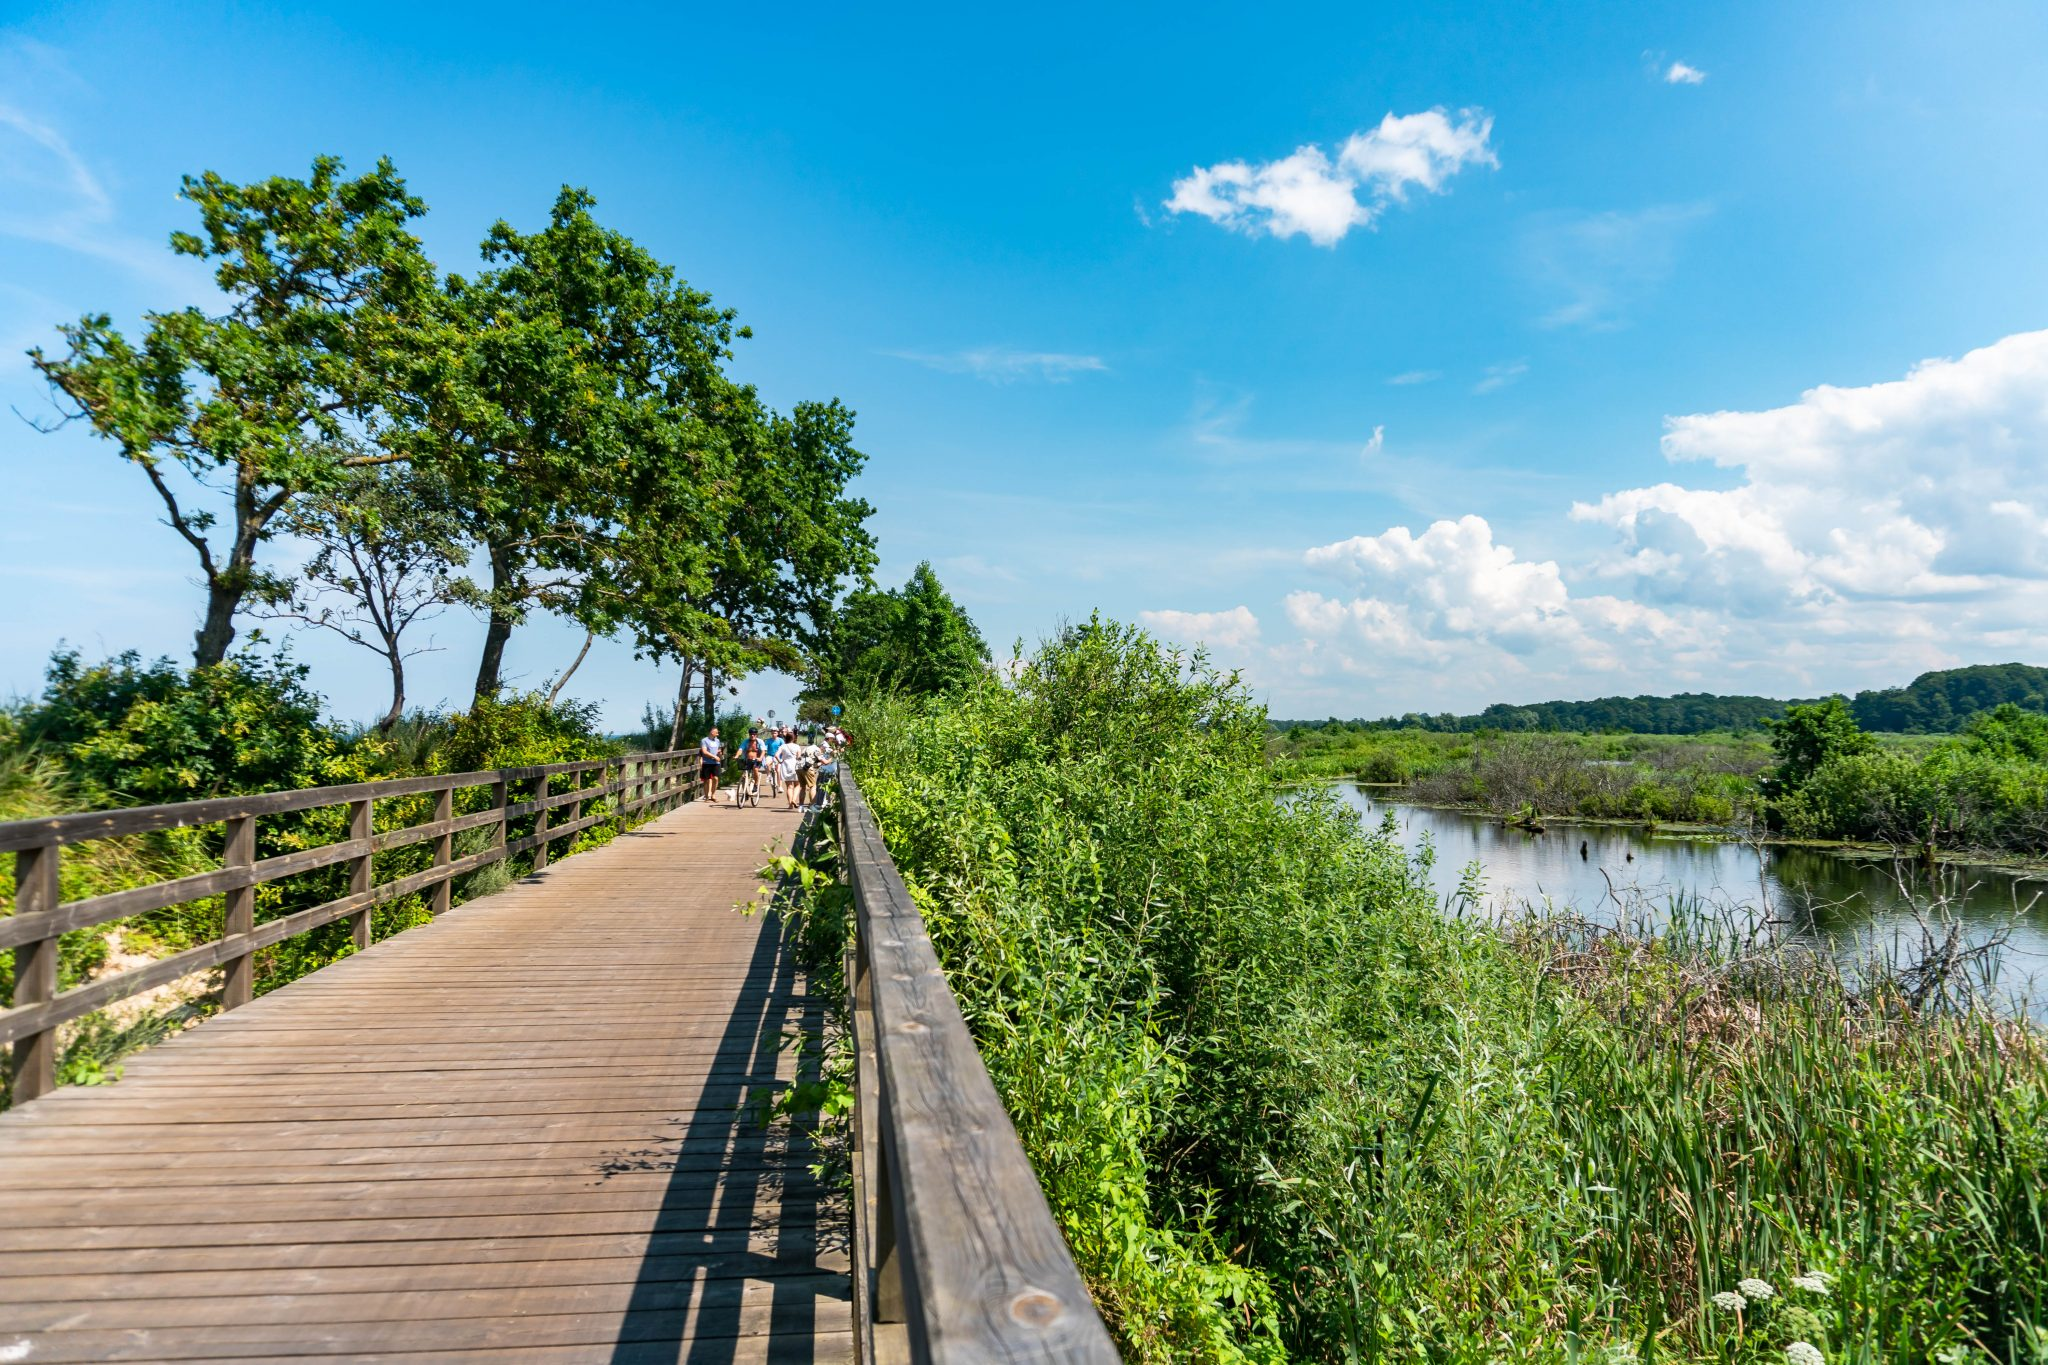
\includegraphics[width=1.05\linewidth]{figures/ekopark_wschodni} 

}

\caption{Ekopark wschodni (Źródło: https://krajewscywpodrozy.pl/wp-content/uploads/2021/07/Rejs-statkiem-Kolobrzeg-2-scaled.jpg)}\label{fig:ryc12}
\end{figure}

\hypertarget{klimat}{%
\section{Klimat}\label{klimat}}

Istotną dla rozwoju turystyki oraz dla rozwoju portu morskiego jest szczególny klimat, którym cieszy się Kołobrzeg.
Kołobrzeg znajduje się w krainie klimatycznej Trzebiatowskiej i Kołobrzesko-Darłowskiej przez co cechuje się większą ilością dni z dużym zachmurzeniem oraz większymi opadami atmosferycznymi.
Temperatura w okresie od maja do lipca jest względnie niższa- występuje mniej dni gorących.
Natomiast zima oraz przymrozki zaczynają się późno i nie wiele jest dni zimowych z utrzymującą się pokrywą śnieżną.
Powyższe cechy klimatyczne sprawiają, że Kołobrzeg jest miastem o jednym z najniższych średnich rocznych amplitud klimatycznych w Polsce \autocite{strategia_promocji}.
Warunki te za sprawą ocieplenia klimatu zmieniają się, jednak wydaje się że niska roczna amplituda temperatur pozostanie cechą charakterystyczną Kołobrzegu, co sugerują badania pod redakcją Joanny Wbig oraz Ewy Jakusik \autocite{wibig}, według których zwiększa się średnia częstość odczucia cieplnego „ciepło'', „bardzo ciepło'' latem i wiosną oraz zmniejsza się częstość odczuć przeciwnych w zimę.

\begin{figure}[t]

{\centering \includegraphics[width=1.05\linewidth]{figures/tabela_klimatu} 

}

\caption{Tabela klimatu dla Kołobrzegu (Źródło: wikipedia.org)}\label{fig:ryc11}
\end{figure}

\hypertarget{inf_trans}{%
\section{Infrastruktura transportowa}\label{inf_trans}}

Kołobrzeg jest korzystnie usytuowany pod względem komunikacyjnym.
Posiadając połączenia drogowe i kolejowe z innymi regionami kraju.
Do Kołobrzegu prowadzą drogi krajowe i ekspresowe (S6, S11, DK11), wojewódzkie (102, 163), powiatowe oraz gminne.
Istnieje dobrze rozwinięta sieć połączeń kolejowych, do Kołobrzegu można się dostać koleją bezpośrednimi pociągami między innymi ze Szczecina, Koszalina, Gdańska, Warszawy i Poznania.

Transport zbiorowy na terenie miasta Kołobrzeg realizowany jest za pośrednictwem Komunikacji Miejskiej w Kołobrzegu Sp. z o.o. (ul. Solna 2), której właścicielem jest Gmina Miejska Kołobrzeg.
Obecnie na terenie miasta funkcjonuje 11 linii autobusowych, na które bilety można zakupić tradycyjnie w formie papierowej, a także poprzez aplikacje mobilne oraz poprzez płatność Kołobrzeską Kartą Mieszkańca.

W pobliżu Kołobrzegu funkcjonuje lotnisko Kołobrzeg-Bagicz, jest to cywilne lotnisko o charakterze sezonowym- czynne od 1 czerwca do 30 września.
W 2015 z kołobrzeskiego lotniska skorzystało 300 samolotów, głównie lekkie samoloty zabierające do 10 pasażerów.
Najbliższy port lotniczy znajduje się w Goleniowie, do którego istnieje połączenie szynobusem z Kołobrzegu (\textcite{lotnisko}).

W planach władz lokalnych jest przebudowanie sieci komunikacyjnej w mieście w celu lepszego połączenia najważniejszych dzielnic miasta z dworcem kolejowym- stworzenie centrum przesiadkowego, skoordynowanego czasowo z transportem publicznym oraz skomunikowanie z parkingami buforowymi oraz centrami handlowymi.

Dużym problemem w zakresie infrastruktury transportowej jest obciążenie lokalnego układu komunikacyjnego przez indywidualny transport kołowy w sezonie turystycznym.
Powoduje to nadmierną eksploatację systemu dróg i powstawanie zjawiska kongestii (natężenie ruchu przekracza przepustowość infrastruktury), co ma wpływ na jakość nawierzchni drogowych, stan infrastruktury towarzyszącej oraz nasilające się negatywne skutki nadmiernego ruchu komunikacyjnego dla środowiska i mieszkańców.
Z problemem tym związany jest deficyt miejsc parkingowych.
Rozwiązaniem tego problemu jest rozwój komunikacji publicznej, w tym rowerowej.
Ta choć generalnie dobrze rozwinięta jest często, nie dostatecznie znana wśród przyjezdnych (\textcite{smartcity}).

\hypertarget{rower_M}{%
\subsection{Informacja o Rowerze Miejskim (historia, cennik, ilość rowerów, mapa)}\label{rower_M}}

W 2016 roku miasto Kołobrzeg uchwaliło \emph{Studium rozwoju infrastruktury rowerowej w Kołobrzegu}, dokument został opracowany przez krakowski oddział stowarzyszenia inżynierów i techników komunikacji.
Jednym z zaleceń studium rowerowego było powstanie roweru miejskiego.
Zalecenie to zostało zrealizowane w 2017 roku.
Obsługą rowerów miejskich zajmuje się firma NextBike.
W 2018 roku powstała stacja sponsorska ``Park Handlowy Albatros'', dysponująca 10 rowerami i będąca pierwsza, jak dotychczas jedyną stacją rowerową powstałą dzięki zaangażowaniu podmiotu prywatnego.
Na terenie miasta do 2020 roku znajdowało się 13 stacji rowerowych (patrz Rycina \ref{fig:ryc9}), a system roweru miejskiego dysponował 135 rowerami - 10 rowerów ``Park Handlowy Albatros'' (patrz Rycina 2.9) (\textcite{kolobrzeskirower}).
Lokalizacje stacji rowerowych jest uzasadniona, stacje znajdują się w bliskiej odległości do terenów rekreacyjnych (parki, stadion/amfiteatr) oraz przy ważnych węzłach komunikacyjnych (patrz Rycina \ref{fig:ryc9}) .

\begin{figure}[t]

{\centering \includegraphics[width=1.05\linewidth]{figures/Kołobrzeg_stacje_git} 

}

\caption{Stacje rowerowe w Kołobrzegu w 2020 roku (Źródło: Opracowanie własne)}(\#fig:rycina29 )
\end{figure}

\begin{figure}[t]

{\centering \includegraphics[width=1.05\linewidth]{figures/stacje_Kol_sat-2} 

}

\caption{Stacje rowerowe w 2020 roku oraz obiekty rekreacyjne (Źródło: Opracowanie własne)}\label{fig:ryc9}
\end{figure}

Obecnie (2021) stacja ``Park Handlowy Albatros'' jest nieczynna, a więc użytkownicy roweru miejskiego dysponują pierwotną liczbą 12 stacji oraz 125 rowerami miejskimi.

Cena za korzystanie z usług Kołobrzeskiego Roweru Miejskiego zależy od posiadania Kołobrzeskiej Karty Mieszkańca.
kołobrzeżaninie mogą korzystać do 40 minut za darmo, czas ten umożliwia w praktyce dostanie się za darmo do dowolnej stacji w Kołobrzegu (w tym do oddalonej stacji Podczele). Powyżej 40 minut a do godziny cena wynosi 2zł, do dwóch godzin 3 zł, natomiast każda kolejna godzina kosztuje 10 zł.
Cennik dla osoby nie posiadającej Kołobrzeskiej Karty Mieszkańca jest podobny z tą różnicą, że przejazd bez opłat jest do 20 minut.
Przed korzystaniem z roweru miejskiego należy uiścić opłate inicjalną w wysokości 10 zł (\textcite{kolobrzeskirower}).

\hypertarget{inf_rower}{%
\subsection{Infrastruktura rowerowa}\label{inf_rower}}

Infrastruktura rowerowa to wszystkie podstawowe urządzenia, usprawnienia służące obsłudze ruchu rowerowego.
Dzieli się na twardą, miękką oraz niewidzialną.
Infrastruktura rowerowa twarda to taka, która obejmuje konkretne rozwiązania dla rowerzystów- wydzielone ścieżki rowerowe, sygnalizacja dla rowerzystów, stojaki i parkingi rowerowe itp.
Infrastruktura miękka to taka, która wprowadza rozwiązania dla rowerów za pomocą oznakowania poziomego.
Infrastruktura niewidzialna to rodzaj infrastruktury rowerowej, którego podstawową funkcją jest służenie innym członkom ruchu drogowego, który uwzględnia jednocześnie potrzeby rowerzystów.
Przykładem niewidzialnej infrastruktury rowerowej są ronda z jednym pasem ruchu, dzięki czemu eliminuje się lewoskręty, będące jedną z najczęstszych przyczyn wypadków rowerowych.
Innym przykładem takich rozwiązań są ograniczenia prędkości do 30 km/h oraz strefy mieszkalne wyrównujące prędkość samochodów do rowerzystów (\textcite{stojaknarower}).

Kołobrzeg jako miasto posiada optymalne warunki do rozwoju ruchu rowerowego:

\begin{itemize}
\item
  płaskie ukształtowanie terenu,
\item
  nie zanieczyszczone powietrze,
\item
  dużą liczbę turystów odwiedzających miasto przez cały rok,
\item
  skalę gwarantującą odległość pomiędzy celem i źródłem podróży nie
  przekraczającą 4km (1)
\end{itemize}

Miasto Kołobrzeg pod względem infrastruktury rowerowej twardej wypada dość dobrze w porównaniu do innych miast w Polsce- istnieje relatywnie rozwinięta sieć dróg rowerowych. Miasto sukcesywnie przy przebudowach ulic stawia nowe stojaki rowerowe - w 2020 roku przy przebudowie ul. Zwycięzców, ul. 18 Marca (\textcite{raport_2020}).
Powstające ścieżki spełniają zalecenia studium rowerowego- zbudowane są z masy mineralno--asfaltowej, rezygnacja z kątów prostych na rzecz łuków itp.

Przez wybrzeże Kołobrzegu prowadzi szlak rowerowy R-10 (\emph{Nadmorski Szlak Hanzeatycki}), który biegnie od Świnoujścia aż do Helu i jest częścią międzynarodowego szlaku EuroVelo. Na rozbudowę transgranicznej ścieżki, w tym zamontowanie liczników umożliwiających pomiar ruchu rowerowego miasto Kołobrzeg współpracuje z gminami ościennymi oraz gminami zagranicznymi w ramach pozyskania środków z Europejskiego Funduszu Rozwoju Regionalnego (\textcite{raport_2019}).

\begin{enumerate}
\def\labelenumi{(\arabic{enumi})}
\tightlist
\item
\end{enumerate}

\hypertarget{gosp}{%
\section{Charakterystyka gospodarcza miasta}\label{gosp}}

Kołobrzeg jest miastem o długiej historii turystyczno-uzdrowiskowej (patrz Rozdział \ref{historia}) co wynika z położenia i zasobów naturalnych (złoża borowiny, wody mineralnej i solanki).
Obecnie na terenie miasta znajdują się 21 uzdrowisk (2019), zapewniające ponad 6200 miejsc noclegowych.
O charakterze Kołobrzegu i jego turystycznej funkcji świadczy ponad 17600 miejsc noclegowych co wpływa na wysoki wskaźnik zasobów mieszkaniowych na 1000 mieszkańców -- 548 mieszkań, przy średniej polskiej 386 mieszkań (2018).
Wartość na sukcesywnie rosła w latach 2012-2019, adekwatnie do liczby turystów -z 350 856 do 591 985 (\textcite{smartcity}).

Mieszkańcy Kołobrzegu wyróżniają się przedsiębiorczością, na terenie gminy jest znacznie więcej firm zajmujących się handlem i naprawami (sekcja G) oraz świadczących usługi gastronomiczne i zakwaterowanie (sekcja I) niż w przeciętnym Polskim mieście.
Wynika to z powiązania firm handlowych z branżą portową oraz firm w sekcji I z branżą turystyczną.
Według badań z 2011 roku ponad 55\% przedsiębiorców uważa Kołobrzeg za dobre miejsce do prowadzenia działalności gospodarczej i tylko niecałe 19\% ocenia Kołobrzeg negatywnie (\textcite{eurotest}).

Kołobrzeg na tle innych miast o znaczącej funkcji turystycznej wyróżnia się wysokim odsetkiem osób pracujący w sektorze usług, który sukcesywnie rósł- z 66,3\% w 2014 roku do 67,9\% w 2018 (\textcite{smartcity}).

Strukturalny charakter gospodarki Kołobrzegu okazał się wrażliwy na zaburzenia przepływu osób i towarów spowodowane Covid-19.
Bezrobocie w 2020 roku wzrosło czterokrotnie w porównaniu z rokiem poprzednim.
Sukces uzdrowiskowy i turystyczny Kołobrzegu ``zaciemnił'' możliwość rozwoju branż opartych na korzystnej lokalizacji nadmorskiej, funkcji logistycznej, czy też w branży innowacyjnej - Kołobrzeg cechuje niski udział podmiotów sektora kreatywnego.
Jest to spowodowane wysokimi kosztami życia mieszkańców miasta, wąskim profilem gospodarczym Kołobrzegu oraz brakiem wyższej uczelni co spowodowało odpływ młodych ludzi.

\hypertarget{analizy}{%
\chapter{Wyniki analiz wypożyczeń rowerów i ankiet}\label{analizy}}

\hypertarget{analiza_wyp}{%
\section{Analiza wypożyczeń}\label{analiza_wyp}}

Analizie poddano dane z sezonu rowerowego 2021, czyli w przedziale czasowym od marca do września 2021 roku.
Dzięki transformacji i eksploracji danych uzyskano informacje o kierunkach przemieszczeń, popularności danych stacji, połączeniach wychodzących i przychodzących w zależności od pory dnia oraz o ilości wypożyczeń w zależności od godziny i dnia oraz w zależności dnia tygodnia bądź miesiąca.
Informacje o wypożyczeniach z poszczególnych miesięcy zgrupowano w wypożyczenia obejmujące cały sezon i poszczególne pory roku - wiosna, lato, jesień.

Największą ilość wypożyczeń zaobserwowano latem, na które przypada 58\% obserwacji, na jesień zaobserwowano ponad 22\% wszystkich obserwacji, natomiast wiosną niecałe 20\% (patrz Rycina \ref{fig:analiza1kol}).
Ilość wypożyczeń właściwie o każdej porze roku spada we wtorek, jest to najbardziej widoczne jesienią, jednak ogólna tendencja widoczna jest przez cały sezon.
W okresie od piątku do niedzieli zaobserwowano wzrost ilości wypożyczeń, co wiąże się najprawdopodobniej z funkcją rekreacyjną roweru miejskiego.
Latem rower miejski jest wykorzystywany z podobną częstotliwością od niedzieli do czwartku, natomiast w piątek i sobotę jest obserwowany wzrost.
Wiosną szczyt wypożyczeń przypada na weekend i od poniedziałku do czwartku następował systematyczny spadek wypożyczeń, tendencja ta zmienia się w piątek, kiedy to następuje trend wzrostowy.

Biorąc pod uwagę wyniki analizy natężenia poszczególnych stacji z uwzględnieniem pór roku oraz biorąc pod uwagę ogólne nasilenie ruchu Kołobrzeskiego Roweru Miejskiego w zależności od pór roku, sugeruje się zwiększenie przepustowości stacji Latarnia Morska i Kamienny Szaniec, które są najbardziej obciążonymi stacjami, a stacje te stanowią najpopularniejszy kierunek przemieszczania się użytkowników roweru miejskiego w Kołobrzegu.
Zwiększenie przepustowości stacji można zrealizować między innymi poprzez zwiększenie liczby stojaków na rowery
.
Analizy wykazują, że prace naprawcze i konserwacyjne rowerów optymalnie powinny być prowadzone w czasie niższej aktywność użytkowników Kołobrzeskiego Roweru Miejskiego, czyli w interwale tygodniowym w poniedziałek i wtorek, natomiast w interwale pór roku wiosną, tak aby w czasie największego natężenia ruchu latem była dostępna jak największa ilość sprawnych rowerów miejskich.

\begin{figure}[t]

{\centering 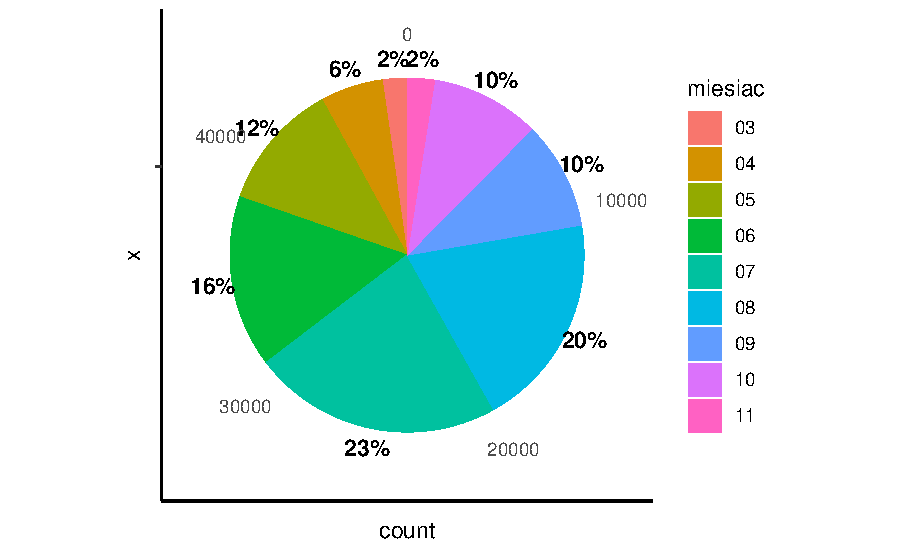
\includegraphics[width=400px]{figures/analiza1kol-1} 

}

\caption{Procentowy udział wypożyczeń w poszczególnych miesiącach  (Źródło: Opracowanie własne)}\label{fig:analiza1kol}
\end{figure}

\begin{figure}[t]

{\centering 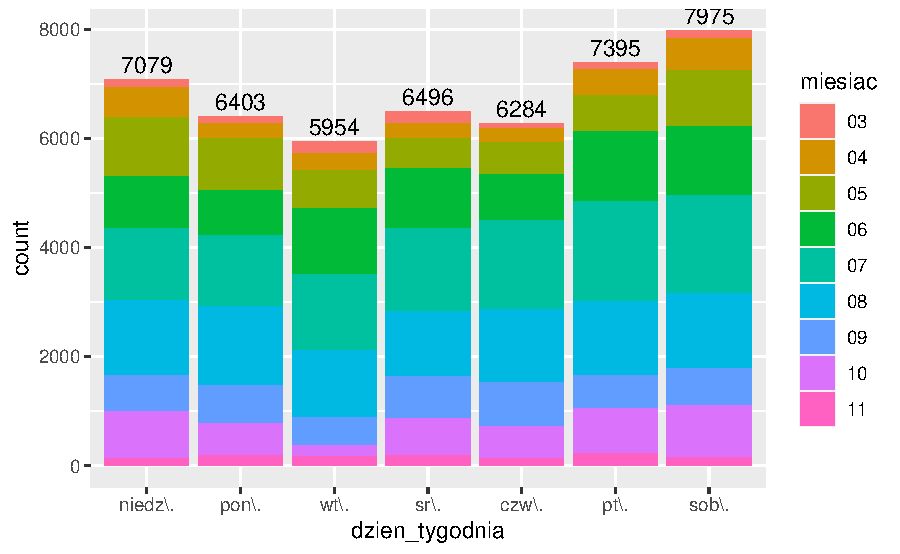
\includegraphics[width=400px]{figures/analiza1p-1} 

}

\caption{Rozklad ilości wypożyczeń w posczególnych dniach tygodnia w sezonie 2021 (Źródło: Opracowanie własne)}\label{fig:analiza1p}
\end{figure}

\begin{figure}[t]

{\centering 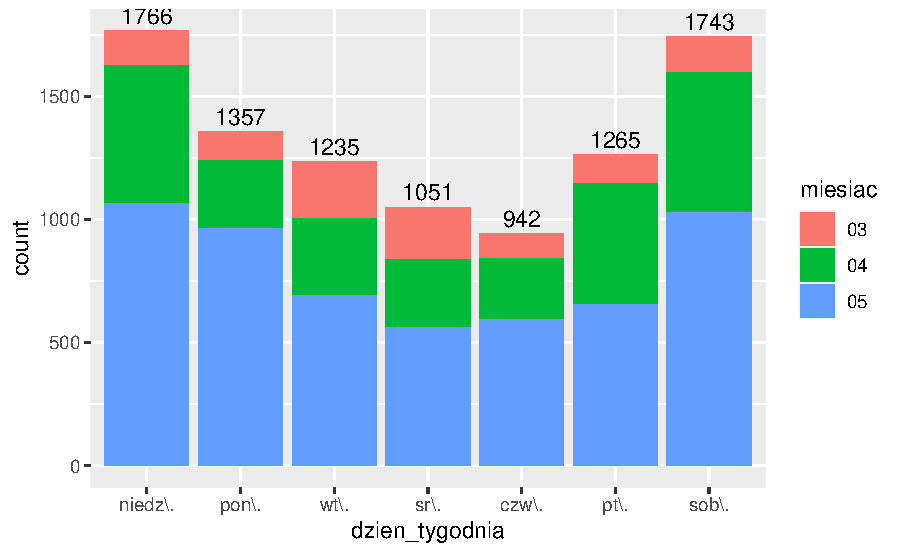
\includegraphics[width=400px]{figures/analiza3-1} 

}

\caption{Wypożyczenia rowerów w poszczególne dni tygodnia wiosną (Źródło: Opracowanie własne)}\label{fig:analiza3}
\end{figure}

\begin{figure}[t]

{\centering 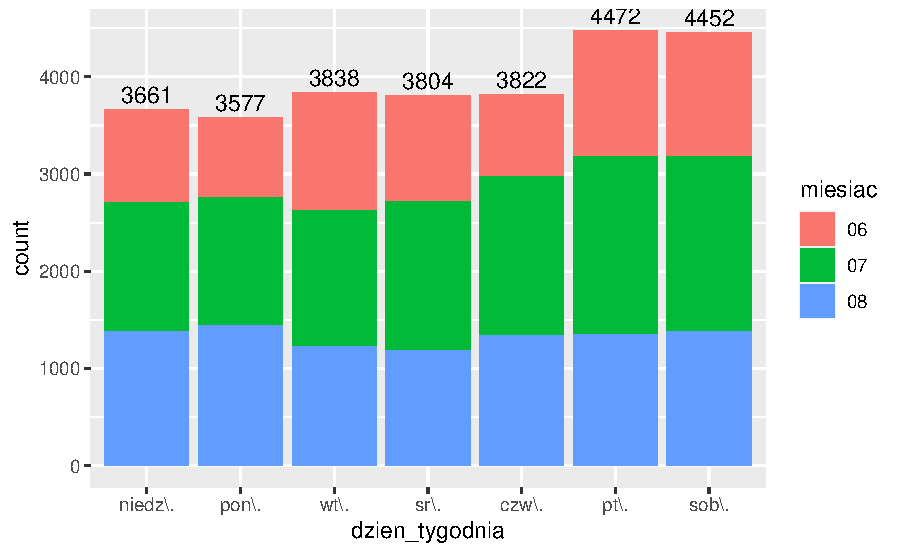
\includegraphics[width=400px]{figures/analiza4-1} 

}

\caption{Wypożyczenia rowerów w poszczególne dni tygodnia latem (Źródło: Opracowanie własne)}\label{fig:analiza4}
\end{figure}

\begin{figure}[t]

{\centering 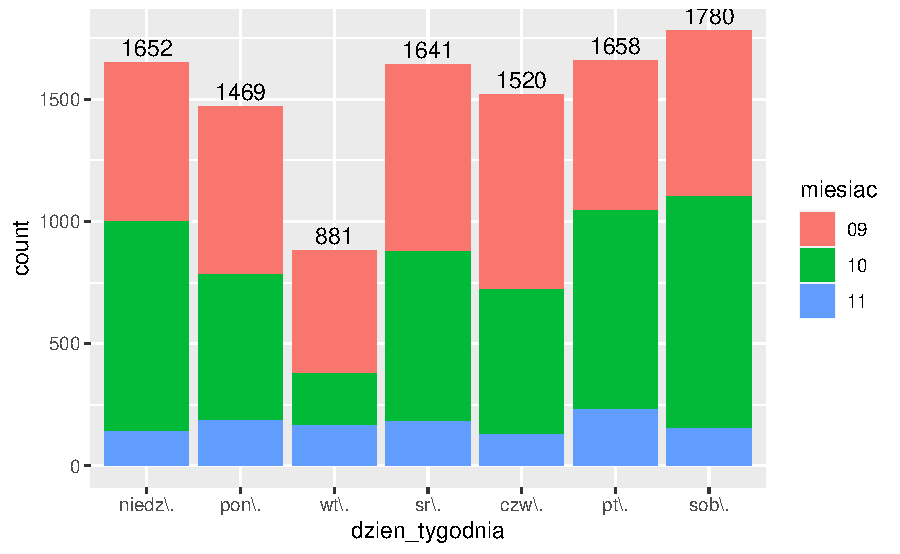
\includegraphics[width=400px]{figures/analiza5-1} 

}

\caption{Wypożyczenia rowerów w poszczególne dni tygodnia jesienią (Źródło: Opracowanie własne)}\label{fig:analiza5}
\end{figure}
\begin{figure}[t]

{\centering 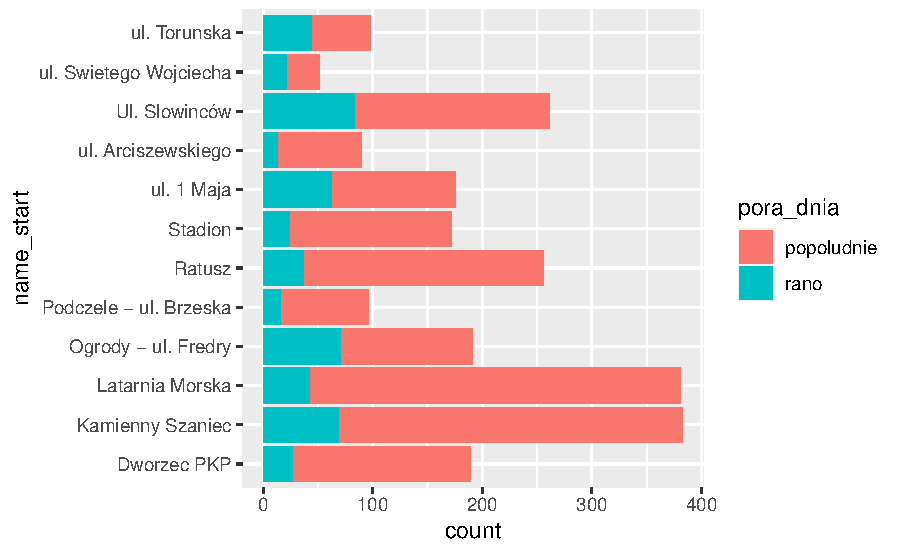
\includegraphics[width=400px]{figures/analiza6-1} 

}

\caption{Wypożyczenia wychodzące w zależności od pory dnia wiosną (Źródło: Opracowanie własne)}\label{fig:analiza6}
\end{figure}

Rano zdefiniowano jako pora dnia od godziny 5 do 9, natomiast popołudnie od godziny 15 do 18.

\begin{figure}[t]

{\centering 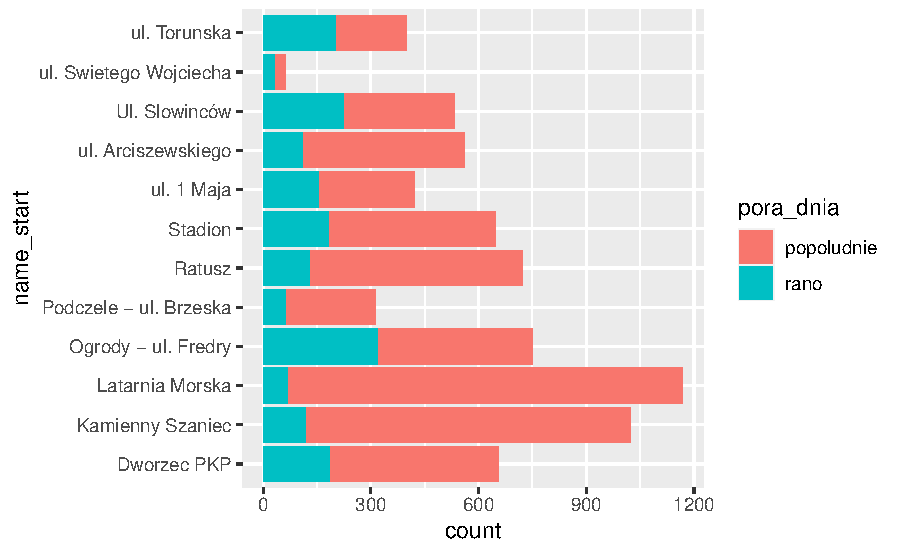
\includegraphics[width=400px]{figures/analiza7-1} 

}

\caption{Wypożyczenia wychodzące w zależności od pory dnia latem (Źródło: Opracowanie własne) }\label{fig:analiza7}
\end{figure}
\begin{figure}[t]

{\centering 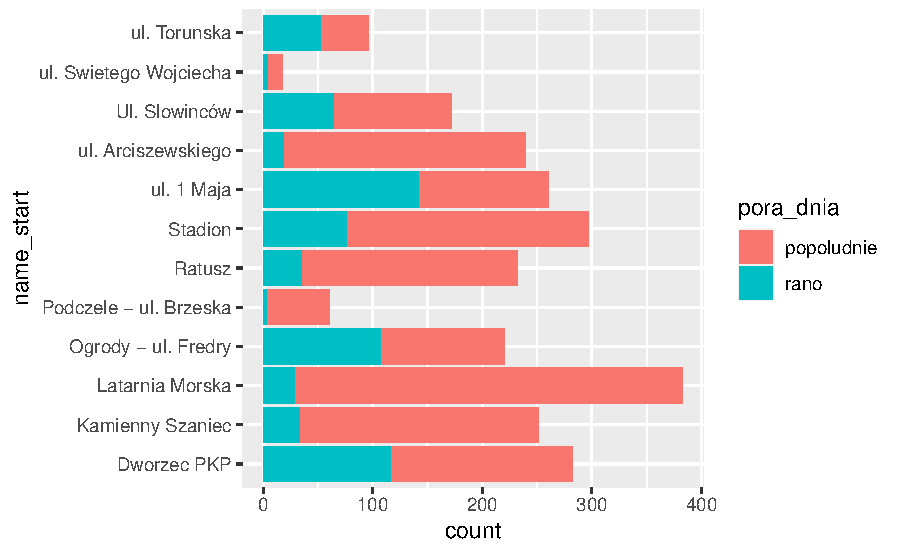
\includegraphics[width=400px]{figures/analiza8-1} 

}

\caption{Wypożyczenia wychodzące w zależności od pory dnia jesienią (Źródło: Opracowanie własne)}\label{fig:analiza8}
\end{figure}

Jesienia można zaobserwowaćwiększy udział wypożyczeń na stacji dworzec PKP oraz

\begin{figure}[t]

{\centering 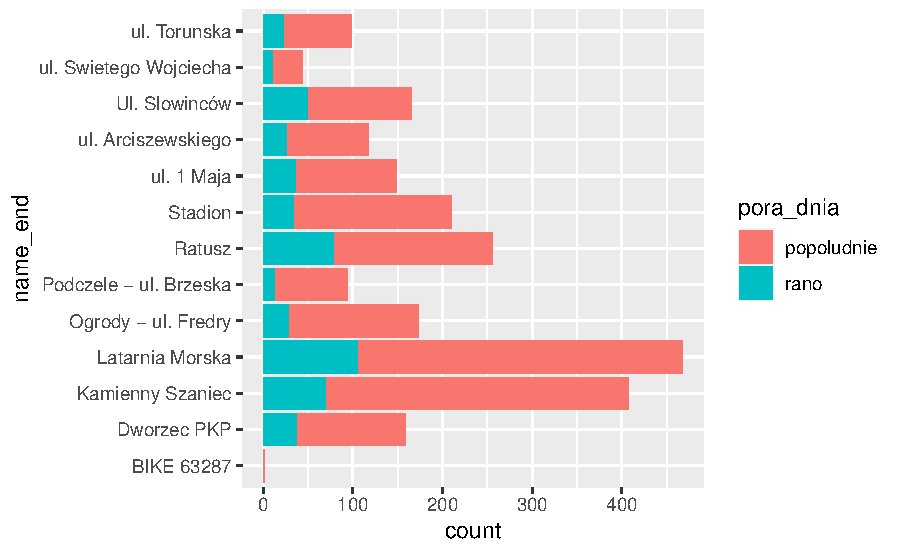
\includegraphics[width=400px]{figures/analiza9-1} 

}

\caption{Wypożyczenia przychodzące w zależności od pory dnia wiosną (Źródło: Opracowanie własne)}\label{fig:analiza9}
\end{figure}

\begin{figure}[t]

{\centering 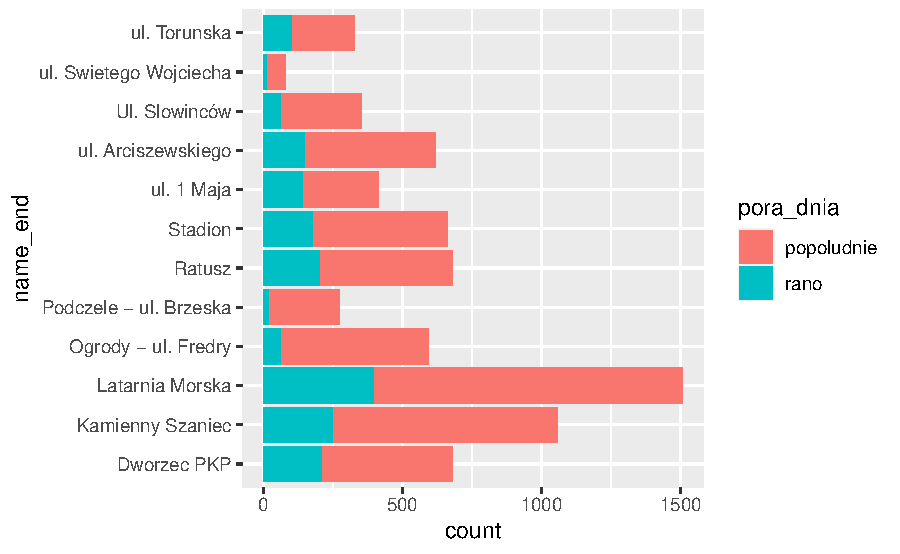
\includegraphics[width=400px]{figures/analiza10-1} 

}

\caption{Wypożyczenia przychodzące w zależności od pory dnia latem (Źródło: Opracowanie własne)}\label{fig:analiza10}
\end{figure}

\begin{figure}[t]

{\centering 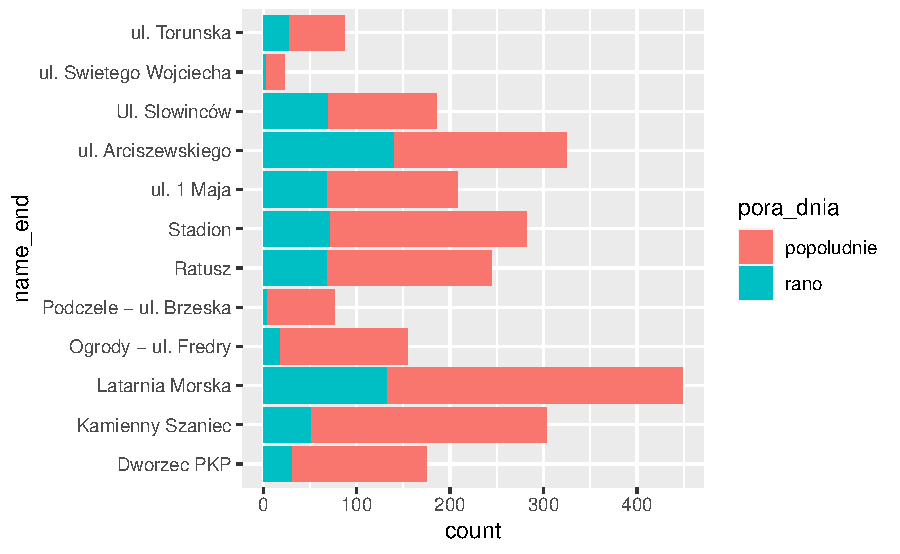
\includegraphics[width=400px]{figures/analiza11-1} 

}

\caption{Wypożyczenia przychodzące w zależności od pory dnia jesienią (Źródło: Opracowanie własne)}\label{fig:analiza11}
\end{figure}

\begin{verbatim}
#> 
#> Dołączanie pakietu: 'dplyr'
#> Następujące obiekty zostały zakryte z 'package:stats':
#> 
#>     filter, lag
#> Następujące obiekty zostały zakryte z 'package:base':
#> 
#>     intersect, setdiff, setequal, union
\end{verbatim}

\begin{figure}[t]

{\centering 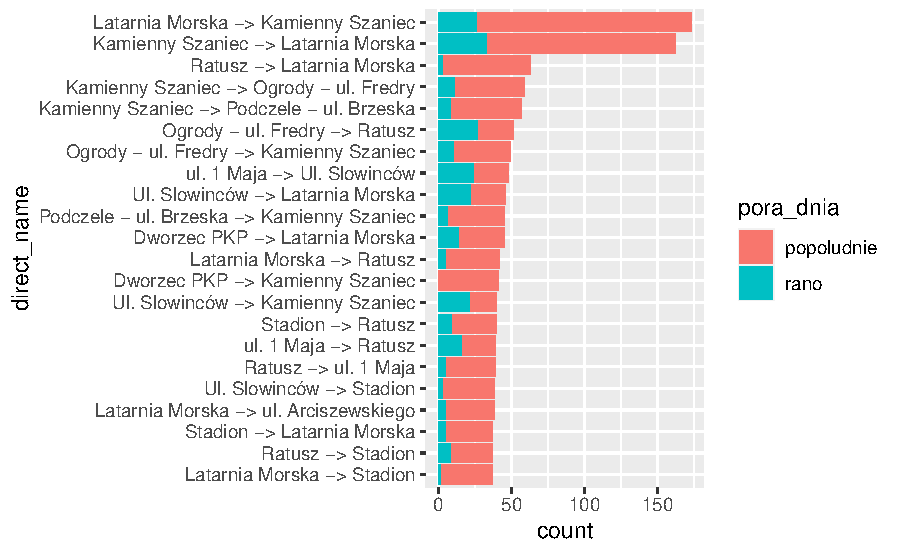
\includegraphics[width=400px]{figures/analiza12-1} 

}

\caption{Najpopularniejsze kierunki w zależności od pory dnia wiosną (Źródło: Opracowanie własne)}\label{fig:analiza12}
\end{figure}
\begin{figure}[t]

{\centering 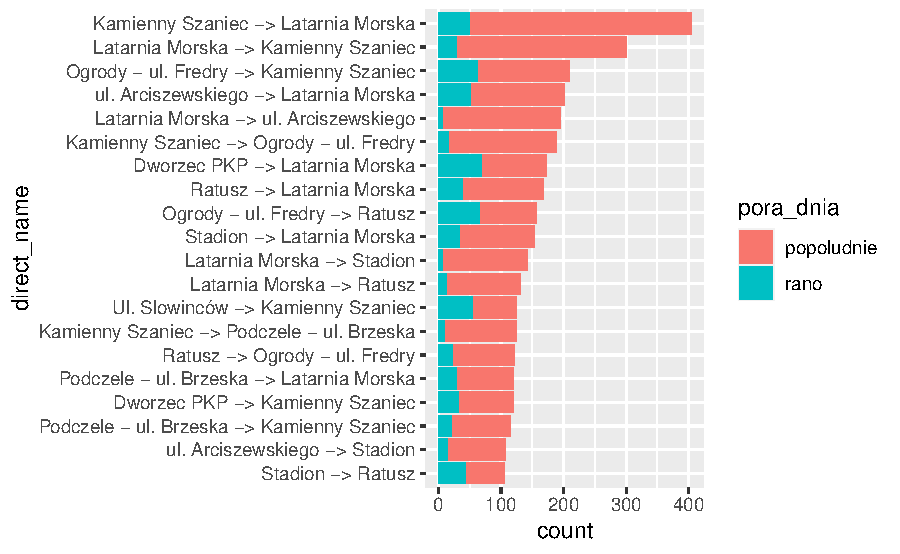
\includegraphics[width=400px]{figures/analiza13-1} 

}

\caption{Najpopularniejsze kierunki w zależności od pory dnia latem (Źródło: Opracowanie własne)}\label{fig:analiza13}
\end{figure}

\begin{figure}[t]

{\centering 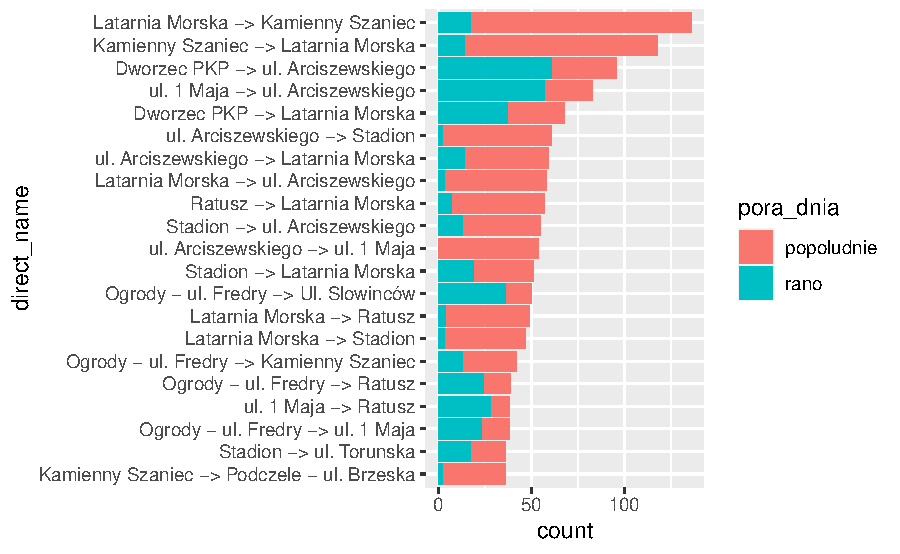
\includegraphics[width=400px]{figures/analiza14-1} 

}

\caption{Najpopularniejsze kierunki w zależności od pory dnia jesienią (Źródło: Opracowanie własne)}\label{fig:analiza14}
\end{figure}
\begin{figure}[t]

{\centering 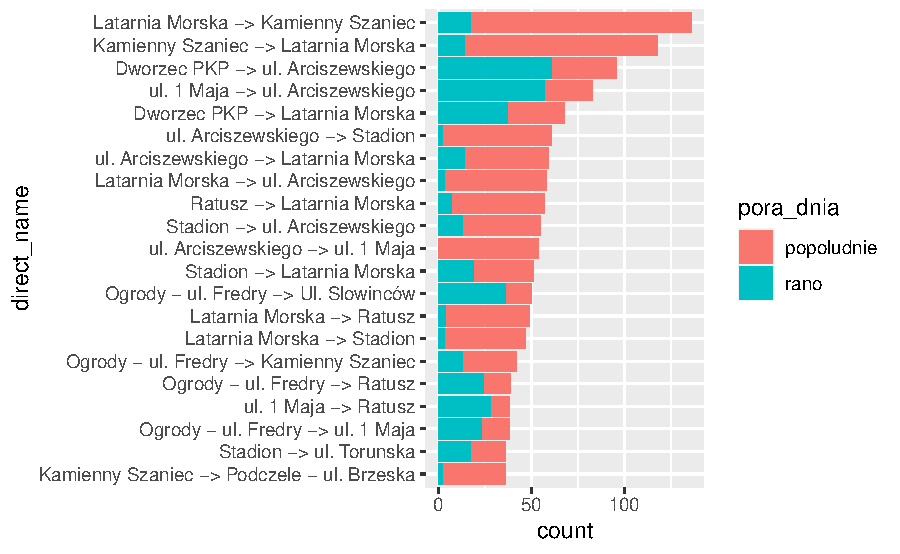
\includegraphics[width=400px]{figures/analiza15-1} 

}

\caption{Najpopularniejsze kierunki w zależności od pory dnia jesienią (Źródło: Opracowanie własne)}\label{fig:analiza15}
\end{figure}

\begin{figure}[t]

{\centering 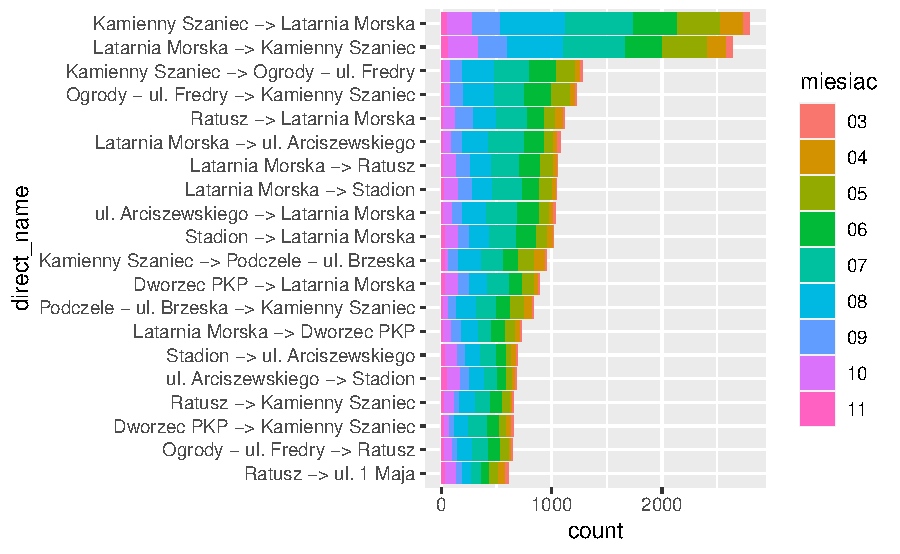
\includegraphics[width=400px]{figures/analiza16-1} 

}

\caption{Najpopularniejsze kierunki w sezonie 2021 (Źródło: Opracowanie własne)}\label{fig:analiza16}
\end{figure}

\hypertarget{ankieta}{%
\section{Badanie ankietowe}\label{ankieta}}

Badanie ankietowe przeprowadzono za pomocą Microsoft Forms.
Kwestionariusz składał się z 10 pytań ogólnych dostępnych dla wszystkich ankietowanych oraz pytań, które dostosowane były do udzielonych przez respondentów odpowiedzi.
Pierwsze rozgałęzienie dotyczy miejsca zamieszkania - respondenci otrzymywali inny zestaw pytań w zależności od ich zamieszkania tz. w Kołobrzegu i okolicach lub poza Kołobrzegiem (powyżej 50 km).
Następnie mieszkańcy Kołobrzegu zostali podzieleni na korzystających z Kołobrzeskiego Roweru Miejskiego oraz tych, którzy dotychczas z niego nie korzystali.
Każda z tych grupo dostała przystosowaną pod nią listę pytań.
Osoby spoza Kołobrzegu były przekierowywane do pytań dla ``turystów'', gdzie następnym kryterium rozgałęzienia był fakt korzystania z roweru miejskiego w Kołobrzegu.
Osobna sekcja pytań do precyzujących dotyczyła osób, które zetknęły się z brakiem rowerów na stacji.
Łącznie kwestionariusz posiadał 40 pytań, natomiast w zależności od odpowiedzi respondenta udzielał on odpowiedzi od 14 do 23 pytań - średnio 18 pytań.
Średni czas jaki respondenci poświęcali na udzielenie odpowiedzi wynosił 3 minuty i 33 sekundy.

Kwestionariusz był dostępny od 8 lipca do 2 września.
Został udostępniony na wybranych grupach społecznościowych portalu Facebook takich jak:

\begin{itemize}
\item
  Forum Mieszkańców Miasta Kołobrzeg
\item
  KOŁOBRZEG
\item
  Wakacje dla seniora
\item
  Rowerem przez Pomorze Zachodnie
\item
  Twoje wakacje nad morzem
\end{itemize}

Odpowiedzi udzieliło 102 respondentów, w tym 38\% mężczyzn i 72\% kobiet (patrz Rycina \ref{fig:ankieta1}).

\begin{figure}[t]

{\centering 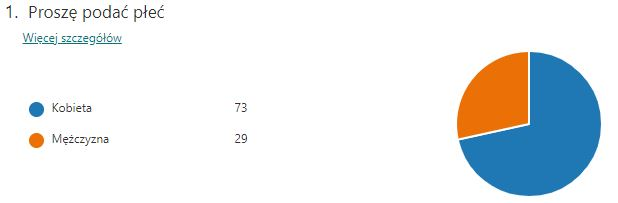
\includegraphics[width=400px]{figures/ankieta/1} 

}

\caption{Struktura płci wśród respondentów (Źródło: Microsoft Forms)}\label{fig:ankieta1}
\end{figure}

Wśród grupy wiekowej respondentów przeważały osoby między 27 a 40 rokiem życia oraz między 41 i 60 rokiem życia, stanowiąc odpowiednio 39\% i 38\% respondentów (patrz Rycina \ref{fig:ankieta2}).
Osoby między 18 a 26 rokiem życia stanowią 13\% respondentów.
Wynika z tego, że 90\% badanych respondentów jest w wieku produkcyjnym (między 18 a 60 rokiem życia) co koreluje z pytaniem czwartym dotyczącym statusu zawodowego, gdzie 72\% osób określiło swój status jako osoby pracujące (patrz Rycina \ref{fig:ankieta4}).
Badanie wykazuje się niską reprezentatywnością osób młodych poniżej 18 roku życia, gdzie prawdopodobną przyczyną jest nie uwzględnienie grup dedykowanych osobom młodym.
Uzyskano dość dobrą reprezentatywność osób po 60 roku życia, biorąc pod uwagę wysokie wykluczenie cyfrowe osób w tym wieku.
Badanie ankietowe ukazuje więc

\begin{figure}[t]

{\centering 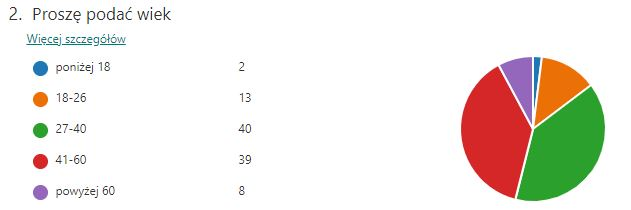
\includegraphics[width=400px]{figures/ankieta/2} 

}

\caption{Struktura wieku wśród respondentów (Źródło: Microsoft Forms)}\label{fig:ankieta2}
\end{figure}

Większość respondentów (56\%) posiada wykształcenie wyższe, wynika to z charakteru badania za pośrednictwem internetu, gdzie według badań osoby z wyższym wykształceniem są bardziej chętne na udział w ankietach. (\emph{to było w tym co dostałem}).
25\% wykształcenie średnie, 11 \% policealne, 5\% zawodowe i 3\% podstawowe, co w przybliżeniu odpowiada respondentom poniżej 18 roku życia (patrz Rycina \ref{fig:ankieta3}).

\begin{figure}[t]

{\centering 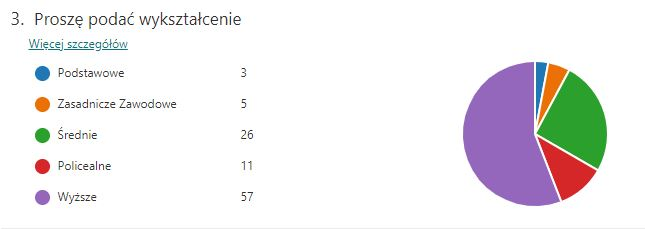
\includegraphics[width=400px]{figures/ankieta/3} 

}

\caption{Struktura wykształcenia wśród respondentów (Źródło: Microsoft Forms)}\label{fig:ankieta3}
\end{figure}

Pod względem statusu zawodowego większość stanowią osoby pracujące (72\%). Liczba osób na emeryturze pokrywa się z liczbą osób po 60 roku życia, przy czym w pytaniu tym możliwe było zaznaczenie kilku odpowiedzi- jest więc prawdopodobne, że część respondentów emerytów równocześnie pracuje. Liczba osób studiujących jest dość niska, porównując z ponad dwukrotnie większą liczbą osób w wieku od 18 do 26 roku życia (patrz Rycina \ref{fig:ankieta4}).

\begin{figure}[t]

{\centering 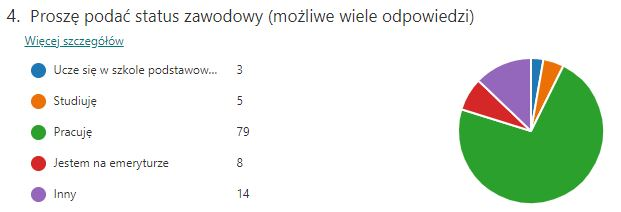
\includegraphics[width=400px]{figures/ankieta/4} 

}

\caption{Status zawodowy wśród respondentów (Źródło: Microsoft Forms)}\label{fig:ankieta4}
\end{figure}

Zdecydowana większość respondentów posiada własny rower (82\%), jest to wysoki wynik. Średnio niecałe 62\% polskich gospodarstw domowych posiada rower (\textcite{gosp_rower}).
Spośród osób posiadających własny rower 92\% osób słyszało o Kołobrzeskim rowerze miejskim (patrz Rycina \ref{fig:ankieta5}).

\begin{figure}[t]

{\centering 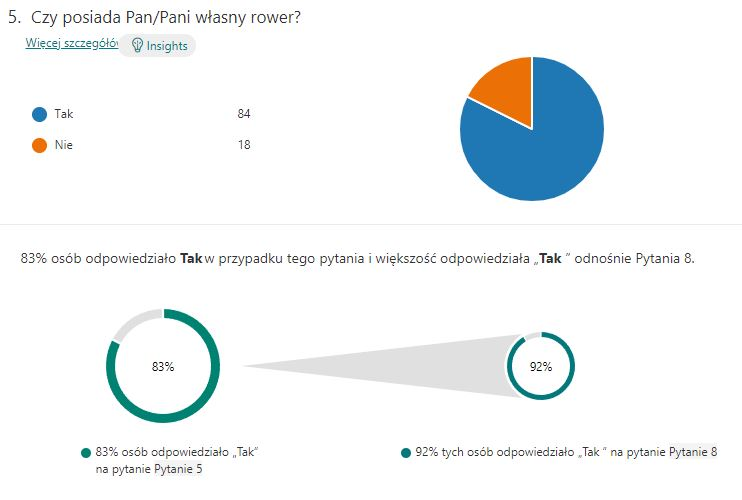
\includegraphics[width=400px]{figures/ankieta/5} 

}

\caption{Posiadanie prywatnego roweru wśród respondentów (Źródło: Microsoft Forms)}\label{fig:ankieta5}
\end{figure}

Większość osób badanych korzysta z roweru dość rzadko, 34\% ankietowanych korzysta z roweru rzadziej niż raz w miesiącu, natomiast kilka razy w miesiącu jeździ 29\% respondentów.
Te dwie grupy stanowią razem 63\% badanych osób.
Kilka razy w tygodniu jeździ 25\% ankietowanych, a 12\% osób jeździ praktycznie codziennie.
Podsumowując grupa aktywnych rowerzystów wśród badanych wynosi 37\% (patrz Rycina \ref{fig:ankieta6}).

\begin{figure}[t]

{\centering 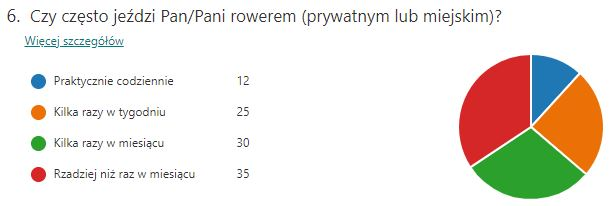
\includegraphics[width=400px]{figures/ankieta/6} 

}

\caption{Częstość podróży wśród respondentów (Źródło: Microsoft Forms)}\label{fig:ankieta6}
\end{figure}

Większośc podróży rowerem wśród respondentów trwa poniżej godziny - 24\% osób badanych podróżuje rowerem do 20 minut, wśród 37\% podróż trwa od 21 minut do godziny.
Podróż trwająca miedzy jedną a dwiema godzinami jest deklarowana przez 25\% respondentów, natomiast podróż powyżej dwóch godzin deklaruje 15\% ankietowanych.
Wśród osób, których podróż rowerem zwykle trwa ponad 2 godziny wszyscy posiadają własny rower. Sugeruje to, że docelowo rower miejski powinien być przeznaczony dla osób, których średnia podróż rowerem jest krótsza co podkreśla teoria oraz uzyskane wyniki analiz (patrz Rycina \ref{fig:ankieta7}).

\begin{figure}[t]

{\centering 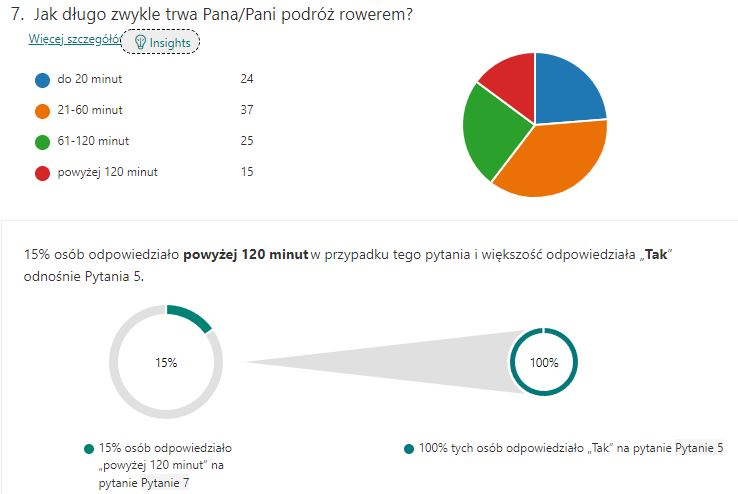
\includegraphics[width=400px]{figures/ankieta/7} 

}

\caption{Czas trwania podróży rowerem wśród respondentów (Źródło: Microsoft Forms)}\label{fig:ankieta7}
\end{figure}

Większość badanych (92\%) słyszała o Kołobrzeskim Rowerze Miejskim\\
(patrz Rycina \ref{fig:ankieta8}), przy czym wszyscy mieszkańcy Kołobrzegu słyszeli o rowerze miejskim (patrz Rycina \ref{fig:ankieta10}).

\begin{figure}[t]

{\centering 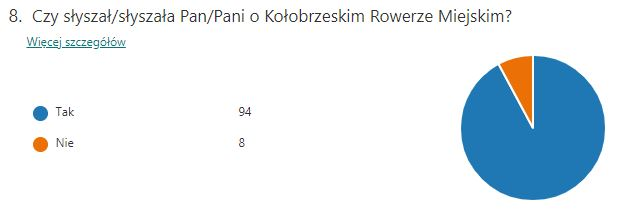
\includegraphics[width=400px]{figures/ankieta/8} 

}

\caption{Znajomość Kołobrzeskiego Roweru Miejskiego wśród respondentów (Źródło: Microsoft Forms)}\label{fig:ankieta8}
\end{figure}

Istotna część (37\%) respondentów deklaruje korzystanie z roweru miejskiego w godzinach 14:00-18:00.
Duża liczba badanych respondentów jeździ od 10 do 14 lub od 18 do 22, odpowiednio 26\% i 27\%.
Respondenci rzadko jeżdżą rano w godzinach 6:00-10:00 (9\%) i bardzo rzadko w godzinach wieczorno-nocnych między 22 a 2 w nocy(patrz Rycina \ref{fig:ankieta9}).

\begin{figure}[t]

{\centering 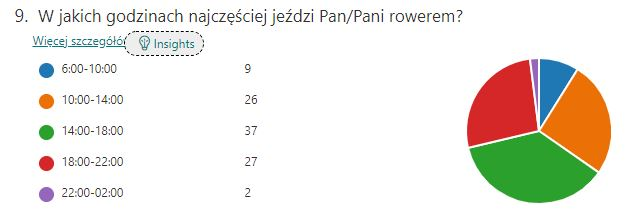
\includegraphics[width=400px]{figures/ankieta/9} 

}

\caption{Godziny podróżowania rowerem wśród respondentów (Źródło: Microsoft Forms)}\label{fig:ankieta9}
\end{figure}

Kolejnym pytanie dotyczyło miejsca zamieszkania.
Wśród respondentów większość (57\%) mieszka na terenie miasta Kołobrzeg, natomiast 17\% w pobliżu Kołobrzegu. Oznacza to, że większość osób badanych to osoby związane z miastem Kołobrzeg.
Natomiast 26\% respondentów to osoby mieszkające powyżej 50 kilometrów od Kołobrzegu.
Założono, że są to osoby odwiedzające Kołobrzeg w celach turystycznych (patrz Rycina \ref{fig:ankieta10}).

\begin{figure}[t]

{\centering 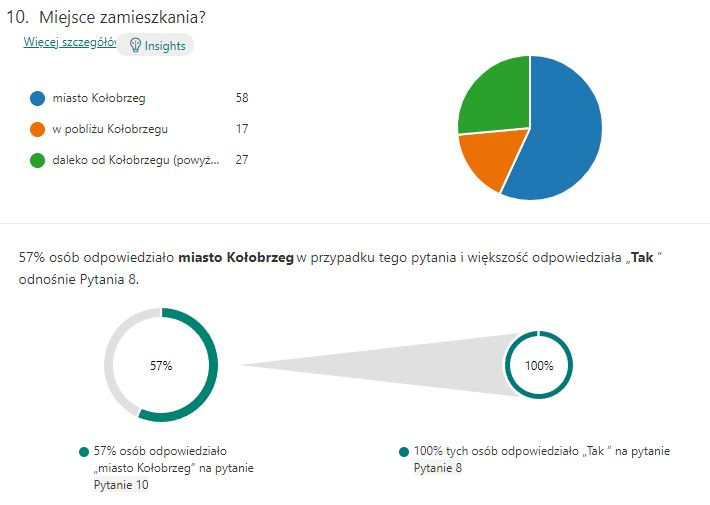
\includegraphics[width=400px]{figures/ankieta/10} 

}

\caption{Miejsce zamieszkania respondentów (Źródło: Microsoft Forms)}\label{fig:ankieta10}
\end{figure}

Wśród ankietowanych mieszkających w Kołobrzegu, bądź w pobliżu Kołobrzegu 51\% respondentów posiada Kołobrzeską Kartę Mieszkańca, natomiast 13\% planuje ją wyrobić.
Karty nie posiada i nie planuje jej wyrobić 36\% ankietowanych (patrz Rycina \ref{fig:ankieta11}).

\begin{figure}[t]

{\centering 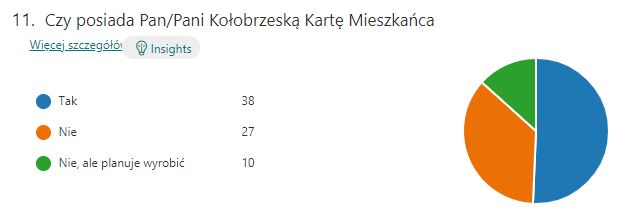
\includegraphics[width=400px]{figures/ankieta/11} 

}

\caption{Posiadanie Kołobrzeskiej Karty Mieszkańca wśród respondentów (Źródło: Microsoft Forms)}\label{fig:ankieta11}
\end{figure}

Z mieszkańców Kołobrzegu lub okolic ponad połowa (52\%) ankietowanych korzystało z Kołobrzeskiego Roweru Miejskiego (patrz Rycina \ref{fig:ankieta12}).
Spośród tych osób większość (44\%) korzysta z roweru miejskiego rzadziej niż raz na miesiąc, 38\% korzysta kilka razy w miesiącu, 13\% kilka razy w tygodniu a 5\% praktycznie codziennie (patrz Rycina \ref{fig:ankieta13}).

\begin{figure}[t]

{\centering 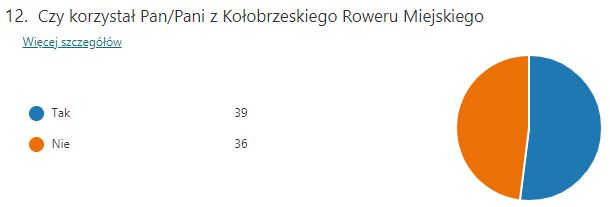
\includegraphics[width=400px]{figures/ankieta/12} 

}

\caption{Korzystający wśród respondentów (Źródło: Microsoft Forms)}\label{fig:ankieta12}
\end{figure}

\begin{figure}[t]

{\centering 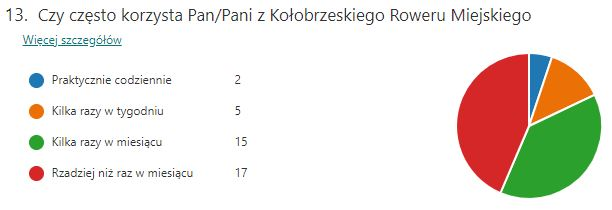
\includegraphics[width=400px]{figures/ankieta/13} 

}

\caption{Struktura częstości korzystania z Kołobrzeskiego Roweru Miejskiego (Źródło: Microsoft Forms)}\label{fig:ankieta13}
\end{figure}

Głównym deklarowanym powodem (46\%) korzystania z roweru miejskiego jest dojazd do ``innych'' miejsc takich jak spotkanie ze znajomymi czy dojechanie do sklepu.
Częstym powodem jest rekreacyjna jazda na rowerze (38\%).
Dojazdy do pracy i dojazdy do szkoły są powodem do korzystania z roweru miejskiego jedynie dla 16\% ankietowanych (patrz Rycina \ref{fig:ankieta14}).

\begin{figure}[t]

{\centering 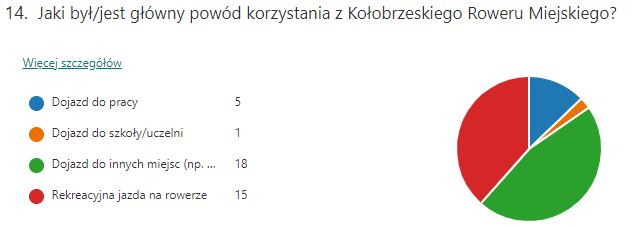
\includegraphics[width=400px]{figures/ankieta/14} 

}

\caption{Główny powód korzystania z KRM deklarowany przez respondentów (Źródło: Microsoft Forms)}\label{fig:ankieta14}
\end{figure}

Jedynie 5\% respondentów korzystało z rowerów z fotelikiem dziecięcym.
Tyle samo procent respondentów korzystało z roweru z fotelikiem w wyniku braku innych rowerów na stacji.

Kołobrzeżanie oceniają kołobrzeski rower miejski na 3.46 w pięciopunktowej skali (patrz Rycina (patrz Rycina \ref{fig:ankieta16}).
Za główna zaletę systemu wymieniają jego dostępność, niski koszt oraz możliwość szybkiego przemieszczania się po mieście.
Z drugiej strony za głównymi wadami Kołobrzeskiego Roweru Miejskiego według respondentów jest zły stan techniczny pojazdów oraz za mała gęstość stacji.
Wielu respondentów zwracało uwagę na błędnie działającą aplikację oraz wadliwe zapięcia na stacjach.
Wielu respondentów (61\%) spotkało się z brakiem wolnego roweru na stacji, przy czym 23\% osób taka sytuacja zdarzyła się często, a 38\% osób miało z nią do czynienia sporadycznie (patrz Rycina \ref{fig:ankieta20}).

\begin{figure}[t]

{\centering 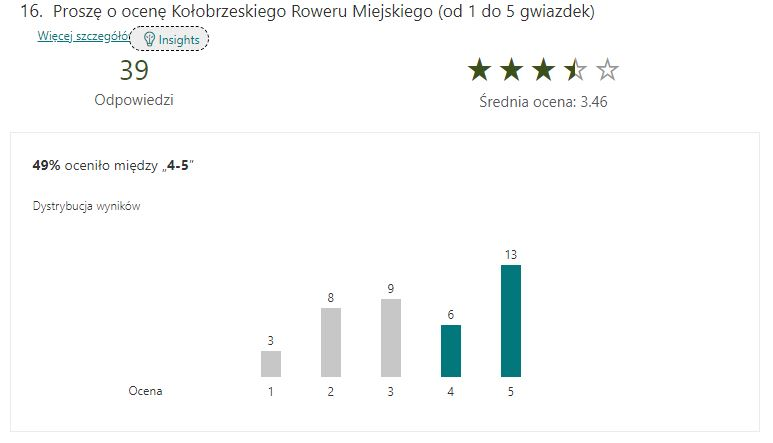
\includegraphics[width=400px]{figures/ankieta/16} 

}

\caption{Ocena Kołobrzeskiego Roweru Miejskiego (Źródło: Microsoft Forms)}\label{fig:ankieta16}
\end{figure}

\begin{figure}[t]

{\centering 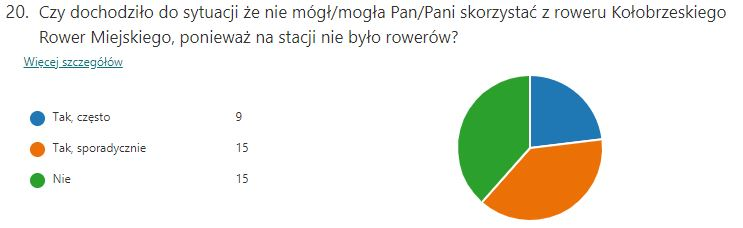
\includegraphics[width=400px]{figures/ankieta/20} 

}

\caption{Brak wolnych rowerów na stacji (Źródło: Microsoft Forms)}\label{fig:ankieta20}
\end{figure}

Spośród mieszkańców, którzy nie korzystali z roweru miejskiego 44\% ankietowanych uważa, że budowa ścieżki rowerowej zdecydowanie spowoduje więcej dojazdów do pracy/szkoły, a 36\% jest zdania, że raczej spowoduje więcej dojazdów.(patrz Rycina \ref{fig:ankieta21})
Respondenci proponują budowę nowych ścieżek rowerowych w pobliżu dróg dojazdowych- zwłaszcza w kierunku zachodnim w stronę Grzybowa (proponowana ulica Grzybowa, Plażowa, Jedności Narodowej), ale także drogę rowerową łączącą Dygowo oraz Ustronie Morskie z Kołobrzegiem.
Budowa wymienionych powyżej ścieżek rowerowych była najczęstszą odpowiedzią wśród respondentów.

znaczący głos dotyczył również budowy ścieżki rowerowej i kładki na kanale drzewnym na ul Łopuskiego.
Przy \emph{Dodać przypis do mapy z proponowanymi ścieżkami i stacjami gdy powstanie}

\begin{figure}[t]

{\centering 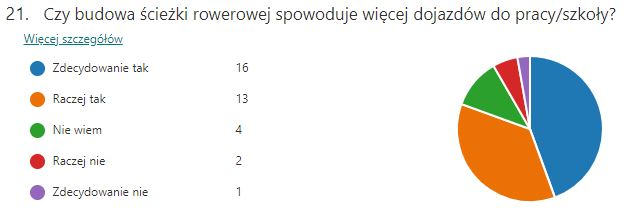
\includegraphics[width=400px]{figures/ankieta/21} 

}

\caption{Zdanie dotyczące korelacji nowych ścieżek rowerowych a dojazdów do pracy wśród responentów (Źródło: Microsoft Forms)}\label{fig:ankieta21}
\end{figure}

Respondenci zostali zapytani czy powstanie stacji rowerowej w korzystnej dla nich lokalizacji spowoduje, że skorzystają oni z Kołobrzeskiego Roweru Miejskiego.
Przeważały głosy niezdecydowane- odpowiedzi ``nie wiem'' udzieliło 31\% ankietowanych, ``raczej tak'' 23\%, ``raczej nie'' 26\%.
Wśród osób zdecydowanych zdecydowanie było więcej głosów przeciwnych - 17\%.
Jedynie jedna osoba (3\%) odpowiedziała zdecydowanie, że powstanie stacji wypożyczeń w korzystnej dla niej lokalizacji spowoduje korzystnie z roweru miejskiego (patrz Rycina \ref{fig:ankieta23}).

Wśród proponowanych nowych stacji wypożyczeń najwięcej ankietowanych skłoniło się ku propozycji stacji w Centrum, oraz ulicy na ulicy Bałtyckiej.
Część propozycji pojawiających się tylko raz zostało odrzucone w drodze analizy, bowiem wiele z proponowanych nowych stacji znajdowała się w odległości mniejszej niż 10 minut pieszo od już istniejących stacji wypożyczeń.
Za realistyczną i potrzebną propozycje stwierdzono stacje wypożyczeń na ulicy wschodniej oraz ewentualnie na ulicy Janiskiej przy rodzinnych ogródkach działkowych.

\begin{figure}[t]

{\centering 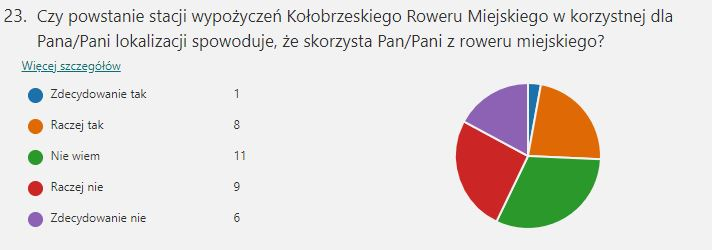
\includegraphics[width=400px]{figures/ankieta/23} 

}

\caption{Zdanie responentów dotyczących ich deklarowanego zachowania jeśli powstanie nowa stacja rowerowa w ich sąsiedztwie (Źródło: Microsoft Forms)}\label{fig:ankieta23}
\end{figure}

Mieszkańcy Kołobrzegu jako główny powód nie korzystania z roweru miejskiego wymieniają posiadanie własnego roweru oraz brak stacji w pobliżu miejsca zamieszkania.
Warto mięć na uwadze wcześniejsze pytanie z którego wynika, że niewielka liczna osób byłaby skłonna korzystać z roweru, jeśli powstałaby nowa stacji w korzystnej dla nich lokacji.

Kołobrzeżanie, nie korzystający z roweru miejskiego podobnie ocenili Kołobrzeski Rower Miejski jak osoby z niego korzystające.
Średnia ocena wynosiła 3.47, natomiast najliczniejszą przyznaną ocena było 3, czyli inaczej niż w przypadku osób korzystających gdzie oceny były inaczej rozlokowane (dominowała ocena 5 z liczną grupą, która wystawiła 2 i 3) w pięciostopniowej skali (patrz Rycina \ref{fig:ankieta26}).

\begin{figure}[t]

{\centering 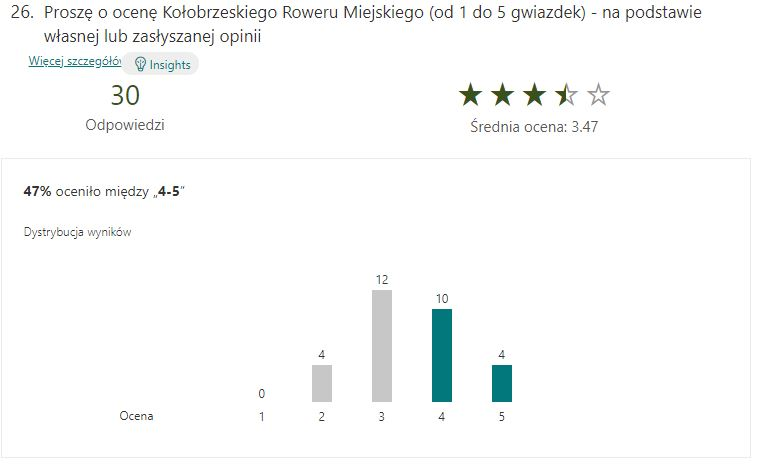
\includegraphics[width=400px]{figures/ankieta/26} 

}

\caption{Ocena KRM przez respondentów nie korzystających z KRM (Źródło: Microsoft Forms)}\label{fig:ankieta26}
\end{figure}

Wśród respondentów mieszkających ponad 50 kilometrów od Kołobrzegu (czyli potencjalni turyści) 81\% ankietowanych nie korzystało z Kołobrzeskiego Roweru Miejskiego.
Oznacza to, że jedynie pięciu ankietowanych ``turystów'' korzystało z roweru miejskiego w Kołobrzegu (patrz Rycina \ref{fig:ankieta27}).
Wskazuje to na konieczność promocji Kołobrzeskiego Roweru Miejskiego wśród przyjezdnych.
Tym bardziej, że zdecydowana większość turystów nie jest zdecydowana czy skorzysta z Kołobrzeskiego Roweru Miejskiego w przyszłości, gdy odwiedzi miasto (patrz Rycina \ref{fig:ankieta35}).
Według ankietowanych turystów skłoniłby do korzystania pierwszy darmowy przejazd, możliwość jazdy bez aplikacji (płatność gotówką lub kartą) oraz lepsza sieć dróg rowerowych w Kołobrzegu.

Większość turystów nie korzysta z roweru miejskiego w swoim miejscu zamieszkania, przy czym turyści, którzy korzystali z KRM częściej korzystali z roweru miejskiego w miejscu zamieszkania (niska próba- 5 osób).

\begin{figure}[t]

{\centering 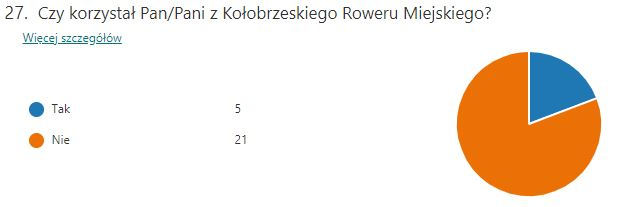
\includegraphics[width=400px]{figures/ankieta/27} 

}

\caption{Korzystanie z KRM przez turystów (Źródło: Microsoft Forms)}\label{fig:ankieta27}
\end{figure}

\begin{figure}[t]

{\centering 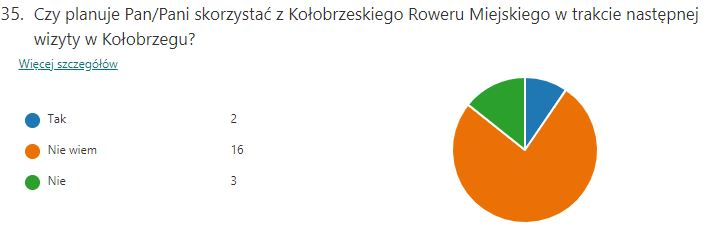
\includegraphics[width=400px]{figures/ankieta/35} 

}

\caption{Planowana podróż KRM przez turystów w czasie następnej wizyty (Źródło: Microsoft Forms)}\label{fig:ankieta35}
\end{figure}

Ankietowani, którzy spotkali się z brakiem rowerów na stacjach wypożyczeń poproszeni zostali o wskazanie stacji na których dochodziło do braków, przy czym możliwe było zaznaczenie wielu stacji.
Brak roweru zaobserwowano wśród ankietowanych na każdej z 12 stacji.
Najczęściej brak rowerów wskazano na stacji ul. Słowieńców i Kamienny Szaniec.
Wśród stacji, gdzie często dochodziło do braków jest ul. 1 Maja, Ratusz, Stadion, Latarnia Morska (patrz Rycina \ref{fig:ankieta38}).
W przypadku, gdy była możliwa tylko jedna odpowiedź i respondenci zostali poproszeni o wskazanie stacji z najgorszą dyspozycyjnością to najczęściej wskazywano stacje na ulicy Słowieńców. (patrz Rycina \ref{fig:ankieta39}).
Zły wynik uzyskały podobne stacje co w poprzednim pytaniu, czyli ul. 1 Maja, Stadion, Ratusz oraz Kamienny Szaniec.
Stacje na ulicy Toruńskiej, Świętego Wojciecha oraz Dworzec PKP tym razem nie zostały wskazane ani razu, co świadczy o generalnie właściwej dyspozycyjności rowerów na tych stacjach.

\begin{figure}[t]

{\centering 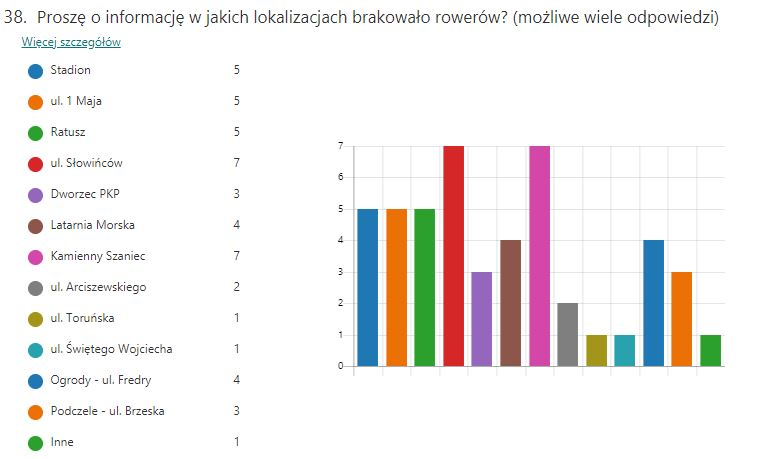
\includegraphics[width=400px]{figures/ankieta/38} 

}

\caption{Brak rowerów- stacje (Źródło: Microsoft Forms)}\label{fig:ankieta38}
\end{figure}

\begin{figure}[t]

{\centering 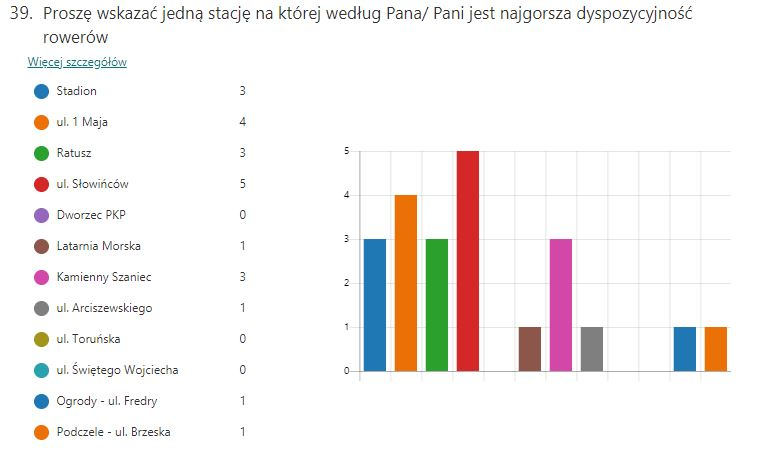
\includegraphics[width=400px]{figures/ankieta/39} 

}

\caption{Stacja o najgorszej dyspozycyjności rowerów (Źródło: Microsoft Forms)}\label{fig:ankieta39}
\end{figure}

\hypertarget{polityka}{%
\chapter{Analiza dokumentów planistycznych i strategicznych}\label{polityka}}

\hypertarget{studium}{%
\section{Studium uwarunkowań i kierunków zagospodarowania przestrzennego}\label{studium}}

Aktualne studium uwarunkowań i kierunków zagospodarowania przestrzennego miasta Kołobrzeg zostało uchwalone przez rade miasta dnia 30 marca 2021 roku.
W części opisowej dokumentu znajdują się informacje dotyczące kształtowania systemu ścieżek rowerowych, zadań systemu komunikacji rowerowej, cech dróg rowerowych, celów układu komunikacji rowerowej oraz powiązania komunikacji rowerowej z komunikacją zbiorową.

W części dotyczącej kształtowania systemu ścieżek rowerowych wymienia się potrzebę powstania systemu ścieżek rowerowych dla mieszkańców oraz turystów pragnących aktywnie spędzać czas. Docelowa długość takiego systemu ścieżek ma wynosić około 40 km, przy czym według studium obecnie wynosi około 15 km i planowana jest budowa 2km odcinka od ulicy Arciszewskiego do Grzybowa oraz od ulicy Brzeskiej do Ustronia Morskiego.
Zauważono, że mimo optymalnej wielkości oraz układu miasta to transport rowerowy w Kołobrzegu jest wykorzystywany głównie w celach rekreacyjnych, a nie jako codzienny środek transportu.

Głównym zadaniem systemu komunikacji rowerowej jest założenie, że 70\% celów i źródeł podróży mieszkańców miasta Kołobrzeg powinno być dostępnych w ramach systemu rowerowego, który jest dobrze zintegrowany z otaczającą go siecią drogową.
System ma się składać z układu tras głównych, które spinają najważniejsze punkty w mieście, tras zbiorczych, wraz z przyjaznym dla ruchu rowerowego śródmieściem oraz z tras dojazdowych i lokalnych.
Rowerowe trasy główne i zbiorcze powinny być oddzielone pasem zieleni.
System rowerowy powinien wpisywać się w projekt europejskiej sieci długodystansowych dróg rowerowych Eurovello.

Wśród cech dróg rowerowych wymieniono odpowiednią nawierzchnię (asfalt, bitumiczną), która umożliwia bezpieczną podróż rowerem o prędkości 30-40 km/godzinę oraz wyznaczenie sieci rowerowej przez praki oraz nadrzeczne bulwary.
Stwierdzono, że do sytemu rowerowego można włączyć istniejące alejki, ścieżki gruntowe, chodniki wzdłuż głównych ulic i pasaże.

Celem układu komunikacji rowerowej w Kołobrzegu jest (\textcite{studium_uwarunkowan}):

\begin{itemize}
\item
  zwiększenie mobilności wszystkich grup wiekowych (dzieci, osoby starsze)
\item
  poprawa mobilności osób bez samochodów i mieszkańców obszarów gorzej, obsługiwanych
  przez komunikację zbiorową,
\item
  zmniejszenie emisji toksycznych (dwutlenek węgla), zmniejszenie zanieczyszczeń środowiska,
\item
  poprawa bezpieczeństwa na drogach (poprzez prowadzenie ruchu rowerowego na wydzielonych
  ścieżkach),
\item
  wykorzystanie roweru w krótkich podróżach po mieście,
\item
  oszczędność miejsc parkingowych dla uczestników ruchu (wskaźnik: 10 rowerów na 1 miejscu
  parkingowym).
\end{itemize}

Powiązanie komunikacji rowerowej z komunikacją zbiorową według studium jest realizowane za pomocą bezpiecznego i komfortowego dojazdu rowerem do głównych przystanków komunikacji zbiorowej oraz do dworców kolejowych, możliwością bezpiecznego przechowywania rowerów na przystankach, możliwością przewozu rowerów środkami komunikacji zbiorowej oraz polityką taryfową sprzyjającą rowerzystom.

\hypertarget{strategia_roz}{%
\section{Strategia rozwoju SmartCity Kołobrzeg}\label{strategia_roz}}

W strategii rozwoju kwestie komunikacji uznawane są za jedno z głównych wyzwań rozwojowych miasta.
związane jest to z bardzo dużym obciążeniem lokalnego układu komunikacyjnego przez indywidualny transport kołowy co nastąpiło wraz z sukcesem turystycznym miasta i ma szczególne znaczenie w sezonie turystycznym.
Według strategii rozwoju długość ścieżek rowerowych w 2018 roku zgodnie z danymi z Głównego Urzędu Statystycznego wynosi 40km, co jest sprzeczne z informacjami przedstawionymi w studium uwarunkowań i kierunków zagospodarowania przestrzennego.

Jednym z priorytetów wymienianych w dokumencie jest \emph{miasto przyjaznej mobilności} gdzie celem jest rozwijanie zrównoważonego i niskoemisyjnego systemu mobilności, opartego na komunikacji publicznej miasta, regionu i kraju, rozwiniętym systemie komunikacji rowerowej oraz na systemach zarządzania. Współgra to z jednym z zadań, które dotyczy stworzenia partycypacyjnego przewodnika miejskiego, który będzie służył między innymi promocji zrównoważonej mobilności w ruchu turystycznym -- sposób formułowania opisów
przemieszczania się powinien w pierwszej kolejności zachęcać do ruchu pieszego, rowerowego
czy korzystania z transportu publicznego.
Zadanie to zostało zrealizowane poprzez udostępnienie aplikacji \emph{Kołobrzeg: RE:GENERACJA}, będącej mobilnym przewodnikiem miejskim, która dostępna jest na smartphone-ach.

W perspektywie realizacji strategii w ramach spójnej i inteligentnej polityki przestrzennej i mieszkaniowej wszystkie kluczowe skupiska zabudowy powinny być położone w zasięgu transportu publicznego i powiązane z siecią dróg dla rowerów.

Sieć rowerowa włączona jest w priorytet miasta ekologicznego w ramach zadania zarządzanie strategiczne błękitno-zieloną siecią dla Kołobrzegu, która oprócz korzyści przyrodniczych ma się wiązać z funkcją społeczno-edukacyjną.

Zwraca się także uwagę na poprawę warunków oświetleniowych rowerzystów w ramach zadania inteligentne i energooszczędne oświetlenie.

Komunikacja rowerowa jest postrzegana w strategii jako jedna z alternatyw (obok transportu miejskiego) dla transportu kołowego.
Uważa się, że należy wzmocnić atrakcyjność komunikacji rowerowej (oprócz rozwoju dróg rowerowych i stacji np. poprzez program zachęt dla pracowników sektora publicznego w zamian za korzystanie z roweru lub transportu publicznego w dojazdach do miejsca pracy), która już teraz posiada duży potencjał, który należy dalej rozwijać poprzez rozwój ścieżek rowerowych oraz usług roweru miejskiego, w tym dążenie do rozszerzenia tych usług w wymiarze funkcjonalnym na sąsiednie gminy w ramach Nadmorskiego Obszaru Funkcjonalnego co jest celem zadania spójna i zintegrowana polityka mobilności dla Kołobrzegu oparta o dane.

Zadanie to jest realizowane, dostępny jest obecnie dobrze rozwinięty system informacji przestrzennej miasta Kołobrzeg dostępny na dedykowanej stronie, gdzie znajdują się dane przestrzenne oraz serwisy mapowe - gdzie można znaleźć miedzy innymi model 3D miasta, ortofotomapy, mapy dotyczące planowania przestrzennego, infrastruktury czy też dostępną mapę strefy płatnego parkowania lub mapę potencjału solarnego dachów.
Możliwość płatności za bilet komunikacji miejskiej oraz parkingowy dostępny jest za pomocą aplikacji Skycash co także jest z zgodne z koncepcją mobilność jako usługa (\textcite{smartcity}).

Strategia stawia także tezę, że inicjatywa Kołobrzeskiego Roweru Miejskiego powinna być stale rozwijana, zarówno w aspekcie zwiększania zasięgu sieci stacji, jak i jej zagęszczenia.

\hypertarget{analiza-swot-w-kontekux15bcie-polityki-przestrzennej-i-infrastruktury-rowerowej}{%
\section{Analiza SWOT w kontekście polityki przestrzennej i infrastruktury rowerowej}\label{analiza-swot-w-kontekux15bcie-polityki-przestrzennej-i-infrastruktury-rowerowej}}

\hypertarget{strengths-mocne-strony}{%
\subsubsection{\texorpdfstring{\emph{Strengths} (Mocne strony)}{Strengths (Mocne strony)}}\label{strengths-mocne-strony}}

\begin{itemize}
\item
  wielkość tkanki miejskiej Kołobrzegu jest optymalna dla ruchu rowerowego
\item
  stosunkowo rozwinięta sieć ścieżek rowerowych
\item
  funkcjonujący Kołobrzeski Rower Miejski
\item
  szlak rowerowy R10 będący częścią europejskiej sieci dróg rowerowych EuroVelo
\item
  wieloletnie działania władz miejskich w kierunku transportu rowerowego (Studium Rowerowe)
\item
  koncepcja Kołobrzeg Smart City
\item
  istniejący system informacji przestrzennej Kołobrzegu
\item
  aplikacja Kołobrzeg RE:GENERACJA
\end{itemize}

\hypertarget{weaknesses-sux142abe-strony}{%
\subsubsection{\texorpdfstring{\emph{Weaknesses} (Słabe strony)}{Weaknesses (Słabe strony)}}\label{weaknesses-sux142abe-strony}}

\begin{itemize}
\item
  obciążenie układu komunikacyjnego przez transport kołowy
\item
  zjawisko kongestii, zwłaszcza w czasie sezonu turystycznego
\item
  brak spójności między strategią a studium
\item
  stan ścieżek rowerowych
\item
  mała gęstość stacji Kołobrzeskiego Roweru Miejskiego
\item
  niska skuteczność promocji korzystania z transportu rowerowego wśród turystów
\end{itemize}

\hypertarget{opportunities-szanse}{%
\subsubsection{\texorpdfstring{\emph{Opportunities} (Szanse)}{Opportunities (Szanse)}}\label{opportunities-szanse}}

\begin{itemize}
\item
  dofinansowanie w ramach Europejskiego Zielonego Ładu
\item
  rozwój współpracy z gminami ościennymi
\item
  wzrastająca świadomość ekologiczna
\item
  inwestycje w ramach rządowego funduszu Polski Ład
\end{itemize}

\hypertarget{threats-zagroux17cenia}{%
\subsubsection{\texorpdfstring{\emph{Threats} (Zagrożenia)}{Threats (Zagrożenia)}}\label{threats-zagroux17cenia}}

\begin{itemize}
\item
  zagrożenia obcięcia budżetu związane z pandemią COVID-19
\item
  wysoka inflacja
\item
  niepewna sytuacja międzynarodowa
\item
  wzrost kosztów towarów na rynku międzynarodowym
\item
  zaburzenia łańcuchu dostaw
\end{itemize}

\hypertarget{koncepcja_zag}{%
\chapter{Koncepcja zagospodarowania}\label{koncepcja_zag}}

\hypertarget{projekt-koncepcji}{%
\section{Projekt koncepcji}\label{projekt-koncepcji}}

Zgodnie z analizą wypożyczeń oraz wynikami ankiet zdecydowano się stworzyć koncepcje, zakładającą rozwój istniejącej sieci stacji roweru miejskiego.

Propozycje stacji:

\begin{itemize}
\item
  Centrum- przy przystanku \emph{Armii Krajowej- poczta}
\item
  ul. Bałtycka- na przystanku \emph{Bałtycka przy Wylotowej}
\item
  ul. Wschodnia - na przystanku \emph{Wschodnia WDW}
\item
  ul. Janiska przy Rodzinnych Ogródkach Działkowych - w pobliżu przystanku \emph{Janiska- osiedle}
\item
  ul. Plażowa - przy Wylotowej w stronę Grzybowa
\end{itemize}

Założeniem projektowym nowych stacji była ich spójność z przystankami komunikacji miejskiej oraz możliwa dostępność terenów zieleni w bliskiej odległości od proponowanej stacji.

\begin{figure}[t]

{\centering \includegraphics[width=1.05\linewidth]{figures/Koł_stacje_git_bezAlbatros_prop} 

}

\caption{Istniejące i proponowane stacje rowere (Źródło: Opracowanie własne)}(\#fig:ryc40 )
\end{figure}

\begin{figure}[t]

{\centering \includegraphics[width=1.05\linewidth]{figures/Koł_stacje_git_bezAlbatros_prop_drogi_row} 

}

\caption{Drogi rowerowe oraz drogi gdzie rowery są dozwolone wraz z isniejącymi oraz proponowanymi stacjami (Źródło: Opracowanie własne)}(\#fig:ryc41 )
\end{figure}

Propozycja jest zgodna z Strategią Smart City dotyczącej obszaru inteligentnej Mobilność i zakładający powstanie spójnej sieci atrakcyjnych ciągów rowerowych oraz z postulatem, że inicjatywa Kołobrzeskiego Roweru Miejskiego powinna być stale rozwijana, zarówno w aspekcie zwiększania zasięgu sieci stacji, jak i jej zagęszczenia.

\begin{figure}[t]

{\centering \includegraphics[width=1.05\linewidth]{figures/mapki_poglad/Bałtycka_l} 

}

\caption{Otoczenie proponowanej stacji Bałtycka, wraz z planem miejscowym- jeśli istnieje (Źródło: Opracowanie własne)}(\#fig:ryc42 )
\end{figure}

Stacja Bałtycka ma znajdować się niedaleko skrzyżowania Bałtyckiej z ulicą Wylotową w pobliżu przystanku autobusowego \emph{Bałtycka przy Wylotowej}. Usytuowana jest korzystnie w drodze ze stacji Stadion na stacje Arciszewskiego (przy jednym z wejść do parku Imienia Jedności Narodowej), jednocześnie będąc 300 metrów od wyżej wymienionego parku. Jest dogodną stacją w drodze na proponowaną stacje Plażową, którą usytuowano także w pobliżu ulicy Wylotowej (patrz Rycina 5.6).

\begin{figure}[t]

{\centering \includegraphics[width=1.05\linewidth]{figures/mapki_poglad/Centrum_l} 

}

\caption{Otoczenie proponowanej stacji Centrum, wraz z planem miejscowym- jeśli istnieje (Źródło: Opracowanie własne)}(\#fig:ryc43 )
\end{figure}

Proponowana stacja Centrum znajduje się w pobliżu przystanku \emph{Armi Krajowej - poczta}, przy placu 18 marca, który otacza stacje. Znajduje się w połowie drogi między istniejącymi stacjami rowerowymi - \emph{Dworzec PKP} i \emph{Ratusz}, a zagęszczenie stacji rowerowych w Centrum było jednym z postulatów wynikających z ankiety przeprowadzonej wśród mieszkańców Kołobrzegu.

\begin{figure}[t]

{\centering \includegraphics[width=1.05\linewidth]{figures/mapki_poglad/Janiska_l} 

}

\caption{Otoczenie proponowanej stacji Janiska, wraz z planem miejscowym- jeśli istnieje (Źródło: Opracowanie własne)}(\#fig:ryc44 )
\end{figure}

Stacja Janiska znajduje się w pobliżu przystanku autobusowego \emph{Janiska osiedle}. Położona jest w sąsiedztwie osiedla na ulicy Rzemieślniczej, rodzinnych ogródków działkowych, terenów zielonych oraz zabudowy o charakterze usługowym od północy. Teren nie jest objęty palnem miejscowym.

\begin{figure}[t]

{\centering \includegraphics[width=1.05\linewidth]{figures/mapki_poglad/Plażowa_l} 

}

\caption{Otoczenie proponowanej stacji Plażowa, wraz z planem miejscowym- jeśli istnieje (Źródło: Opracowanie własne)}(\#fig:ryc45 )
\end{figure}

Stacja Plażowa znajduje się w północno-zachodniej części miasta w pobliżu ulicy Wylotowej, biegnącej w stronę sąsiedniego Grzybowa.
Stacja w kierunku na Grzybowo była jednym z postulatów jakie wynikają z ankiety, a jej położenie w niedalekiej odległości od plaży sugeruje o możliwym dużym natężeniu ruchu rowerowego.
Proponowana stacja znajduje się pobliżu terenów zieleni, stacji ładowania pojazdów elektrycznych oraz zabudowy usługowej- głównie hoteli takich jak \emph{Neptun}, \emph{Sun \& Snow Resorts - Kołobrzeg} i \emph{Baltic Plaza Hotel Medi SPA\&fit}.
W pobliżu znajduje się droga rowerowa prowadząca w stronę drogi rowerowej R-10 oraz nad Plaże Zachodnią Radzikowo.

\begin{figure}[t]

{\centering \includegraphics[width=1.05\linewidth]{figures/mapki_poglad/Wschodnia_l} 

}

\caption{Otoczenie proponowanej stacji Wschodnia, wraz z planem miejscowym- jeśli istnieje (Źródło: Opracowanie własne)}(\#fig:ryc46 )
\end{figure}

Stacja Wschodnia, znajduje się na ulicy Wschodniej biegnącej na osi północ-południe w pobliżu skrzyżowania z Dywizji Wojska Polskiego, która biegnie w stronę centrum miasta.
Ulica wschodnia łączy wiele osiedli z terenem nadmorskim i okolicznymi apartamentami. Proponowana stacja znajduje się w sąsiedztwie osiedla na ulicy Generała maczka oraz niezagospodarowanych terenów zieleni na północy wschód od stacji (głównie tereny bagniste).
W pobliżu stacji znajduje się przystanek autobusowy, Wojskowy Dom Wypoczynkowy oraz tory kolejowe (wraz z kładką pieszo-drogową).
Proponowana stacja znajduje się w optymalnej odległości od pobliskich stacji wypożyczeń Roweru Miejskiego \emph{Kamienny Szaniec} oraz \emph{Ogrody - ulica Fredry}, które zgodnie z analizą (patrz rozdział \ref{analizy}) cechują się dużym natężeniem ruchu rowerowego.

\hypertarget{podsumowanie}{%
\chapter{Podsumowanie}\label{podsumowanie}}

Głównym celem pracy było opracowanie danych pozyskanych za pośrednictwem Nextbike API za pomocą języka R, w celu uzyskania informacji o natężeniu ruchu rowerowego na poszczególnych stacjach Kołobrzeskiego Roweru Miejskiego w zależności od pory roku, miesiąca, dnia, pory dnia oraz uzyskanie informacji o najpopularniejszych przemieszczeniach.
Analizy wzbogacono o ankietę dotyczącą Kołobrzeskiego Roweru Miejskiego oraz miejskiej infrastruktury rowerowej, w której respondenci zostali otrzymali inny zestaw pytań w zależności od charakteru ich relacji z miastem Kołobrzeg- mieszkańcy, turyści.
Przedstawiono charakterystykę miasta - historię, uwarunkowania geograficzno-przyrodnicze, środowiskowe, klimatyczne oraz stan infrastruktury rowerowej i charakterystykę gospodarczą miasta.
Analizie poddano również dokumenty planistyczne i strategiczne, to znaczy studium uwarunkowań i kierunków zagospodarowania przestrzennego oraz strategie rozwoju miasta SmartCity.
Następnie opracowano analizę SWOT (silne,słabe strony, szanse i zagrożenia) w kontekście polityki przestrzennej i infrastruktury rowerowej

Wynikiem analiz jest projekt koncepcji nowych stacji Kołobrzeskiego Roweru Miejskiego wraz z
przedstawieniem nowych stacji rowerowych na mapie miasta Kołobrzeg oraz z przedstawionymi drogami rowerowymi (drogi rowerowe oraz drogi z dopuszczalnym ruchem rowerowym).
Sporządzono także mapy przedstawiające sąsiedztwo proponowanych nowych stacji roweru miejskiego wraz z planem miejscowym, w sytuacji, gdy proponowana stacja znajduje się na terenie lub sąsiedztwie terenu objętego planem miejscowym.

\printbibliography[heading=bibintoc, title=Bibliografia]

\end{document}
